\documentclass[UTF8, Microsoft YaHei]{book}
\usepackage{amsmath}
\usepackage{graphicx}
\usepackage{float}
\usepackage{subfigure}
\usepackage{xeCJK}
\usepackage[colorlinks,linkcolor=blue]{hyperref}
\usepackage{algorithm2e}
\usepackage{amsfonts}
\usepackage{epsfig}
\usepackage{listings}
\usepackage{xcolor}
% 定义可能使用到的颜色

\definecolor{CPPLight}  {HTML} {686868}
\definecolor{CPPSteel}  {HTML} {888888}
\definecolor{CPPDark}   {HTML} {262626}
\definecolor{CPPBlue}   {HTML} {4172A3}
\definecolor{CPPGreen}  {HTML} {487818}
\definecolor{CPPBrown}  {HTML} {A07040}
\definecolor{CPPRed}    {HTML} {AD4D3A}
\definecolor{CPPViolet} {HTML} {7040A0}
\definecolor{CPPGray}  {HTML} {B8B8B8}
\lstset{
    columns=fixed,
    numbers=left,                                        % 在左侧显示行号
    frame=none,                                          % 不显示背景边框
    backgroundcolor=\color[RGB]{245,245,244},            % 设定背景颜色
    keywordstyle=\color[RGB]{40,40,255},                 % 设定关键字颜色
    numberstyle=\footnotesize\color{darkgray},           % 设定行号格式
    commentstyle=\it\color[RGB]{0,96,96},                % 设置代码注释的格式
    stringstyle=\rmfamily\slshape\color[RGB]{128,0,0},   % 设置字符串格式
    showstringspaces=false,                              % 不显示字符串中的空格
    language=c++,                                        % 设置语言
    morekeywords={alignas,continute,friend,register,true,alignof,decltype,goto,
    reinterpret_cast,try,asm,defult,if,return,typedef,auto,delete,inline,short,
    typeid,bool,do,int,signed,typename,break,double,long,sizeof,union,case,
    dynamic_cast,mutable,static,unsigned,catch,else,namespace,static_assert,using,
    char,enum,new,static_cast,virtual,char16_t,char32_t,explict,noexcept,struct,
    void,export,nullptr,switch,volatile,class,extern,operator,template,wchar_t,
    const,false,private,this,while,constexpr,float,protected,thread_local,
    const_cast,for,public,throw,std},
}

\graphicspath{{images/}}
\setCJKmonofont{SimSun}

\title{\Huge{DeepCamera\\}\huge{安卓应用设计实验报告}}
\author{\huge{易凯\\ \\ Email: williamyi96@gmail.com\\ Project Page: https:github.com/WilliamYi96/DeepCamera}}
\date{\huge{2017年6月28日}}

\begin{document}
  \maketitle
  \vspace{15mm}
  % \begin{flushcenter}
  % \Large{
  %   \textbf{班\ \ \ \ \ 级} \makebox[5em][l]{软件53班}

  %   \textbf{学\ \ \ \ \ 号} \makebox[5em][l]{2151601053}

  %   \textbf{邮\ \ \ \ \ 箱} \makebox[5em][l]{williamyi96@gmail.com}

  %   \textbf{联系电话} \makebox[5em][l]{13772103675}

  %   \textbf{项目网站} \makebox[5em][l]{\small{\href{https://github.com/WilliamYi96/DeepCamera}{github.com/WilliamYi96/DeepCamera}}}

  %   \textbf{提交日期} \makebox[5em][l]{2017年4月30日}
  %   }
  %   \end{flushcenter}
    \newpage
    \tableofcontents
    % \newpage
    % \listoffigures
    % \newpage
    % \listoftables
    \newpage

    \chapter{关于本报告的说明}
    \section{致谢}
    Give my sincere thanks to Teacher Du for his excellent teaching skills and serious altitude for our homework. Give my sincere thanks to some students who have helped us and who have inspired us when discussing with them. Give my sincere thanks to myself because I've overcome all difficulties and have successfully finished our embedded-software and android assignments -- DeepCamera. Give my sincere thanks to those pioneers who have devoted themselves to writing immortal books. Give my sincere thanks to all the people sharing their ideas and harvests without pay in QA communities.

    ~

    ~

    衷心感谢杜小智老师出色的教学风范以及严谨的治学态度,衷心感谢那些在讨论中帮助和启发我们的同学们,衷心感谢克服了种种困难最终完成了嵌入式软件与安卓设计综合实验的自己,衷心感谢那些写了不朽著作为后人指明道路的先驱们,衷心感谢那些在问答社区无私奉献自己智慧成果的所有同仁!
    \newpage

    \section{内容声明}
    本实验报告是西安交通大学2015级软件工程系本科生以《嵌入式软件设计与安卓综合实验》设计为契机进行的《Android-Machine Learning: DeepCamera》的设计与实现。所有工作均主要由本人完成。项目设计与实现过程中,严格采取工程模块化的设计思想,务必追求严谨,考虑周全。经过接近一个月的设计与实现,最终于2017年6月末完成整体设计,并完成所有相关代码以及样例运行。

    关于该实验的相关程序以及发布在GitHub上,读者可以下载学习共同探讨心得,

    项目地址为\url{https://github.com/WilliamYi96/DeepCamera}.,欢迎读者提出宝贵意见。
    \newpage

    \section{作者信息}

    易凯,西安交通大学软件工程专业软件53班。学号为2151601053,联系邮箱williamyi96@gmail.com. 主要研究兴趣为深度学习,机器视觉以及增强学习。现于智能网络与网络安全教育部重点实验室,西安交通大学软件学院创新实验室进行科研与工程训练。目前作为负责人完成国家级大学生创新创业训练课题。


    座右铭: 为天地立心,为生灵立命, 为往圣继绝学,为万世开太平!

    ~

    ~

    William Yi, who majors in software engineering in Xi\'an Jiaotong University. He is interested in deep learning, computer vision and reinforcement learning. And he is the intent of Key Laboratory of Intelligent Network and Network Security, Ministry of Education in Xi\'an Jiaotong University. The member of Innovative laboratory in software institute as well. Besides, He is conducting a national student project.

    Motto: Pursue what you want and do want only you can do.

    \chapter{实验研究基本背景}
    \section{基本介绍}
    出于实际需要,实验研究背景部分进行简要说明。

    由于android相对而言操作性更强,因此以下说明内容更多地放在machine learning之上。

    从2012年来,以深度学习(其核心为卷积神经网络CNN和循环神经网络RNN)为代表的机器学习引起了极大的轰动性。由于卷积神经网络与循环神经网络自身的特性,能够大大地提升各个领域的效率,其得到的结果相当惊艳,机器学习已经被应用于自然语言处理,机器视觉,语音识别,甚至是不对称信息博弈(代表为AlphaGo与德州扑克)。

    TensorFlow是google于2015年推出的机器学习平台,一经推出,即引起了很大反响,大大提升了机器学习实践的效率,如何该项目在GitHub上的star数已经超过了6W,成为了机器学习框架中的姣姣者。

    一直以来,目标识别(object detection)就是一个十分棘手的问题,没有任何或者少量先验知识进行物体识别的难度可想而知。而当前,为了有效地提升目标识别的准确度,学者们提出了各种各样的解决方案。

    在这种大背景之下,萌生了将两者进行有机结合来设计制作APP的想法。


    \section{TensorFlow}
    TensorFlow 是一个采用数据流图(data flow graphs),用于数值计算的开源软件库。节点(Nodes)在图中表示数学操作,图中的线(edges)则表示在节点间相互联系的多维数据数组,即张量(tensor)。它灵活的架构让你可以在多种平台上展开计算,例如台式计算机中的一个或多个CPU(或GPU),服务器,移动设备等等。TensorFlow 最初由Google大脑小组(隶属于Google机器智能研究机构)的研究员和工程师们开发出来,用于机器学习和深度神经网络方面的研究,但这个系统的通用性使其也可广泛用于其他计算领域。

    Tensorflow 有一个合理的c++使用界面,也有一个易用的python使用界面来构建和执行我们的graphs。我们可以直接写python/c++程序,也可以用交互式的ipython界面来执行。

    TensorFlow基本情况可以概括为以下几点;

     \begin{itemize}
      \item TensorFlow使用Graph来表示计算任务
      \item 在被称之为Session的context中执行图
      \item 使用tensor表示数据
      \item 使用Variable维护状态
      \item 使用feed和fetch可以为任意操作赋值或者从中获取数据
    \end{itemize}

    该机器学习框架以张量流的形式进行图运算,作为机器学习library中的重要成员,起到了极大作用。
   
    \section{JNI--DNK}
    JNI,是Java Native Interface的缩写,其是一种编程方式,中文为Java本地调用。通俗地说,JNI是一种技术,通过这种技术可以做到以下两点:

    \begin{itemize}
      \item Java程序中的函数可以调用Native语言写的函数,Native一般指的是C/C++编写的函数。
      \item Native程序中的函数可以调用Java层的函数,也就是在C/C++程序中可以调用Java的函数。
    \end{itemize}

    在Android平台上,JNI就是一座将Native世界和Java世界间的天堑变成通途的桥,来看图2-1,它展示了Android平台上JNI所处的位置:

    ~

    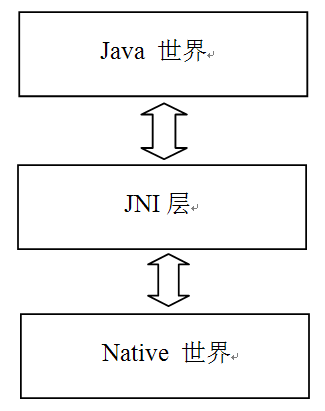
\includegraphics[width=0.6\textwidth]{./img/JNI.png}

    Android的设计开发过程中继承了JNI这种编程方式,同时其发展为NDK。NDK 全称是 Native Development Kit。NDK 提供了一系列的工具,帮助开发者快速开发 C(或C++)的动态库,并能自动将 so 和 java 应用一起打包成 apk。这些工具对开发者的帮助是巨大的。

    \chapter{项目总体设计}
    \section{总体流程图}

    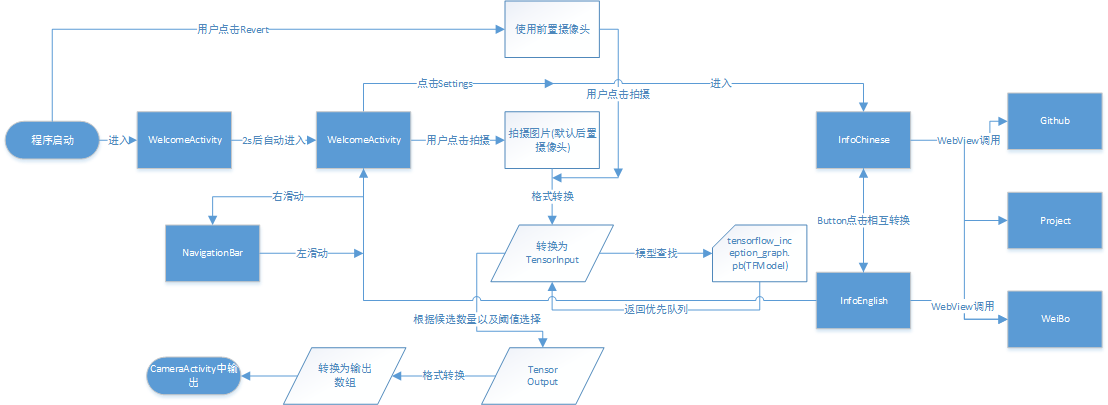
\includegraphics[width=1.0\textwidth]{img/outline.png}

    \section{总体设计描述}

    在系统启动之后,首先进入WelcomeActivity状态,2s之后跳转至MainActivity。

    在MAinActivity中,向右滑动可以进入NavigationBar,然后向左滑动可以撤销上述操作。此外可以选择点击转换相机视角,从后置摄像头拍摄转换为前置摄像头拍摄。如果拍摄按键被执行,则进入模型处理、图片选择阶段。

    图片选择阶段首先获取拍摄的照片,然后再将该照片转换为TensorFlow的Input格式,然后通过内置的模型以及数据标签进行分析,通过优先队列排出结果,然后将输出的结果(Tensor Output Form)转换为数组格式,通过添加的筛选个数以及阈值条件将结果进行输出。

    WelcomeActivity通过点击settings可直接进入到InfoChinese的Activity,该activity中显示的是作者的基本信息。

    InfoChinese有回退键(直接回到MAinActivity),也有切换键,直接进入到英文格式(InfoEnglish), 还可以通过点击button访问作者的Github page, project page和weibo page。 

    \chapter{项目模块化设计}
    \section{TensorFlow模型Android应用}
    我们要将下述内容中编译好了的TensorFlow文件.so导入到Android应用中,然后通过Android的原生文件支持标准.jar文件将.so文件进行解析(.jar文件中存放的是调用cpp的JAVA API)。

    然后再将得到的TensorFlow的Object Detection对应的模型与对应的监督学习模式下的标签导入进来即可。

    同时,注意上述导入过程中创建的项目要允许C++ Support.
    
    \section{Image分类识别实现}
    \subsection{设置选择标准}
    我们仅仅选择通过TensorFlow模型得到的置信度最高的结果,其中最大选择数量为3, 同时设置置信阈值为0.1f。如下所示:

\begin{small}
\begin{lstlisting}[language=java]
private static final int MAX_RESULTS = 3;
private static final float THRESHOLD = 0.1f;
\end{lstlisting}
\end{small}

	\subsection{将物品标签写入内存}

\begin{small}
\begin{lstlisting}[language=java]
String actualFilename = labelFilename.split("file:///android_asset/")[1];
BufferedReader br = null;
br = new BufferedReader(new InputStreamReader(assetManager.open(actualFilename)));
String line;
while ((line = br.readLine()) != null) {
    c.labels.add(line);
}
br.close();
\end{lstlisting}
\end{small}

		recognizeImage方法是实现图片识别的核心,采用的方式具体如下:

	\subsection{将图像数据转换为bitMap支持的数据格式}

	~

	具体的转换关系如下:

\begin{small}
\begin{lstlisting}[language=java]
bitmap.getPixels(intValues, 0, bitmap.getWidth(),
			 0, 0, bitmap.getWidth(), bitmap.getHeight());
    for (int i = 0; i < intValues.length; ++i) {
    final int val = intValues[i];
    floatValues[i * 3 + 0] = (((val >> 16) & 0xFF) - imageMean) / imageStd;
    floatValues[i * 3 + 1] = (((val >> 8) & 0xFF) - imageMean) / imageStd;
    floatValues[i * 3 + 2] = ((val & 0xFF) - imageMean) / imageStd;
}
\end{lstlisting}
\end{small}

	\subsection{将输入的数据导入TensorFlow模型}

\begin{small}
\begin{lstlisting}[language=java]
inferenceInterface.fillNodeFloat(                
    inputName, new int[]{1, inputSize, inputSize, 3}, floatValues);
\end{lstlisting}
\end{small}

	\subsection{运行模型推理得到输出tensor}

\begin{small}
\begin{lstlisting}[language=java]
inferenceInterface.runInference(outputNames);
\end{lstlisting}
\end{small}

	\subsection{将输出Tensor转变为输出数组}

\begin{small}
\begin{lstlisting}[language=java]
inferenceInterface.readNodeFloat(outputName, outputs);
\end{lstlisting}
\end{small}

	\subsection{找到最佳匹配的图片}

~

首先通过优先队列进行TensorFlowFlow库中图片置信度选择:

\begin{small}
\begin{lstlisting}[language=java]
PriorityQueue<Recognition> pq =
    new PriorityQueue<Recognition>(
        3,
        new Comparator<Recognition>() {
        @Override
        public int compare(Recognition lhs, Recognition rhs) {
          return Float.compare(rhs.getConfidence(), lhs.getConfidence());
        }
    });
......
\end{lstlisting}
\end{small}


然后按照优先队列的顺序将大于阈值的图片输出筛选出来,如果没有,则输出为unknown,若有则最多输出三个:

\begin{small}
\begin{lstlisting}[language=java]
for (int i = 0; i < outputs.length; ++i) {
  if (outputs[i] > THRESHOLD) {
    pq.add(
      new Recognition(
        "" + i, labels.size() > i ? labels.get(i) :
        	 "unknown", outputs[i], null));
  }
}
\end{lstlisting}
\end{small}

通过如下方式进行数量比对:
\begin{small}
\begin{lstlisting}[language=java]
int recognitionsSize = Math.min(pq.size(), MAX_RESULTS);
\end{lstlisting}
\end{small}

	最后将结果调用poll()函数输出即可。
    
    \section{WelcomeActivity}
   	欢迎模块实现的是应用程序启动时进入WelcomeActivity欢迎界面,经过2s延时之后进入MainActivity页面。其中可以通过在WelcomeActivity中使用Thread和Handler进行控制延时和启动。

   	\subsection{将WelcomeActivity声明为默认启动}

   	默认的启动方式是从MainActivity中启动,将其改为从WelcomeActivity中启动即可。修改的地方是AndroidManifest.xml.

\begin{small}
\begin{lstlisting}[language=java]
<activity android:name=".WelcomeActivity">
  <intent-filter>
    <action android:name="android.intent.action.MAIN" />
    <category android:name="android.intent.category.LAUNCHER" />
  </intent-filter>
</activity>
\end{lstlisting}
\end{small}

    \subsection{自定义启动页面基本内容}

    自定义启动主体是LinearLayout,其中采用的启动背景画面是welcome.png, 启动时定义了两个TextView,内容分别为DeepCamera 和 Android with Tensorflow.

    具体的参数如下:


\begin{small}
\begin{lstlisting}[language=xml]
<?xml version="1.0" encoding="utf-8"?>
<LinearLayout xmlns:android="http://schemas.android.com/apk/res/android"
    xmlns:tools="http://schemas.android.com/tools"
    android:id="@+id/activity_welcome"
    android:layout_width="match_parent"
    android:layout_height="match_parent"
    android:background="@drawable/welcome"
    android:orientation="vertical"
    tools:context="com.deepcamera.williamyi.welcometest.WelcomeActivity">

<TextView
   android:text="DeepCamera"
   android:layout_width="match_parent"
   android:layout_height="wrap_content"
   android:textAlignment="center"
   android:textColor="@android:color/holo_orange_light"
   android:textSize="45dp"
   android:layout_marginTop="100dp"
   android:layout_alignParentTop="true"
   android:layout_alignParentLeft="true"
   android:layout_alignParentStart="true"
   android:id="@+id/textView1" />
<TextView
   android:text="Android with Tensorflow"
   android:layout_width="match_parent"
   android:layout_height="wrap_content"
   android:textAlignment="center"
   android:textColor="@android:color/holo_orange_light"
   android:textSize="35dp"
   android:layout_marginTop="10dp"
   android:layout_alignParentTop="true"
   android:layout_alignParentLeft="true"
   android:layout_alignParentStart="true"
   android:id="@+id/textView2" />
</LinearLayout>
\end{lstlisting}
\end{small}

    \subsection{使用Handler进行Activity切换}
    使用Handler进行Activity切换,并制定睡眠时间为2s,同时使用到了isShowWelcom(), 便于之后进行是否显示WelcomeActivity的设置。

\begin{small}
\begin{lstlisting}[language=java]
handler=new Handler(){
@Override
public void handleMessage(Message msg) {
    Intent intent=new Intent(WelcomeActivity.this,MainActivity.class);
    startActivity(intent);
    WelcomeActivity.this.finish();
    }
};

if(!isShowWelcome(this)) {
    Intent intent=new Intent(this,MainActivity.class);
    startActivity(intent);
    this.finish();
}   else{
    new Thread(){
    @Override
    public void run() {
    try {
        Thread.sleep(2000);
        handler.sendEmptyMessage(0);
    } catch (InterruptedException e) {
        e.printStackTrace();
        }
      }
    }.start();
}
\end{lstlisting}
\end{small}

    \section{ToolBar and NavigationBar}
    ToolBar和NavigationBar都是MaterialDesign中的内容,其联合使用可以大大增强安卓UI的整体效果。

    \subsection{自定义ActionBar}
    由于任何新建的项目,默认都是会显示ActionBar,但是ActionBar较为传统,灵活度不高。因此我们若想用Meterial Design中的内容,则需要在style中更改主题。

    修改为如下所示:

\begin{small}
\begin{lstlisting}[language=xml]
<resources>

<!-- Base application theme. -->
<style name="AppTheme" parent="Theme.AppCompat.Light.NoActionBar">
    <!-- Customize your theme here. -->
    <item name="colorPrimary">@color/colorPrimary</item>
    <item name="colorPrimaryDark">@color/colorPrimaryDark</item>
    <item name="colorAccent">@color/colorAccent</item>
</style>

</resources>
\end{lstlisting}
\end{small}

	以上操作完成之后我们就成功地将ActionBar隐藏起来了,接下来修改activity\_main.java中的代码,用ToolBar代替ActionBar.

	修改完成之后的内容如下所示:

\begin{small}
\begin{lstlisting}[language=xml]
<?xml version="1.0" encoding="utf-8"?>
<FrameLayout xmlns:android="http://schemas.android.com/apk/res/android"
    xmlns:app="http://schemas.android.com/apk/res-auto"
    xmlns:tools="http://schemas.android.com/tools"
    android:layout_width="match_parent"
    android:layout_height="match_parent"
    tools:context="com.deepcamera.williamyi.welcometest.MainActivity">

    <android.support.v7.widget.Toolbar
        android:id="@+id/toolbar"
        android:layout_width="match_parent"
        android:layout_height="?attr/actionBarSize"
        android:background="@color/colorPrimary"
        android:theme="@style/ThemeOverlay.AppCompat.Dark.ActionBar"
        app:popupTheme="@style/ThemeOverlay.AppCompat.Light">
    </android.support.v7.widget.Toolbar>

</FrameLayout>
\end{lstlisting}
\end{small}

	\subsection{将xml插件传给MainActivity}

	通过findViewById()得到Toolbar的实例,然后调用setSupportActionBar()方并将ToolBar实例传入,我们及可以使用ToolBar并且保持其外观上的一致。

	\subsection{丰富toolbar}
	在res目录之下新建menu,同时在文件夹下新建toolbar.xml文件,自定义toolbar中显示的内容。

	如下所示:

\begin{small}
\begin{lstlisting}[language=xml]
<?xml version="1.0" encoding="utf-8"?>
<menu xmlns:android="http://schemas.android.com/apk/res/android"
    xmlns:app="http://schemas.android.com/apk/res-auto">
    <item
        android:id="@+id/backup"
        android:icon="@drawable/ic_backup"
        android:title="Backup"
        app:showAsAction="always"/>
    <item
        android:id="@+id/delete"
        android:icon="@drawable/ic_delete"
        android:title="Delete"
        app:showAsAction="ifRoom"/>
    <item
        android:id="@+id/settings"
        android:icon="@drawable/ic_settings"
        android:title="Settings"
        app:showAsAction="never"/>
</menu>
\end{lstlisting}
\end{small}

	接下来我们调用onCreateOptionMenu()方法,并加载toolbar.xml菜单文件,然后在onOptionsItemSelected()方法中处理各个按钮的点击事件。

	如下所示:

\begin{small}
\begin{lstlisting}[language=java]
public boolean onCreateOptionsMenu(Menu menu) {
    getMenuInflater().inflate(R.menu.toolbar, menu);
    return true;
}

@Override
public boolean onOptionsItemSelected(MenuItem item) {
    switch (item.getItemId()) {
    case android.R.id.home:
        mDrawerLayout.openDrawer(GravityCompat.START);
        break;
    case R.id.backup:
        Toast.makeText(this, "You clicked Backup",
        Toast.LENGTH_SHORT).show();
        break;
    case R.id.delete:
        Toast.makeText(this, "You clicked Delete",
        Toast.LENGTH_SHORT).show();
        break;
    case R.id.settings:
        Toast.makeText(this, "You clicked Settings",
        Toast.LENGTH_SHORT).show();
        break;
    default:
    }
    return true;
}
\end{lstlisting}
\end{small}

	关于NavigationBar由于Android Studio自身的特性,无需进行额外的设置,新建activity时直接选择Navigation FrameLayout即可。

    \section{Camera}
    \subsection{定制CameraView}
    Camera的UI由四个部分构成,分别为CameraView, ImageViewResult, ToggleButton 和Object Detection Button。

    其中CameraView采取的是一般化的布局,如下所示:

\begin{small}
\begin{lstlisting}[language=xml]
<com.flurgle.camerakit.CameraView
    android:id="@+id/cameraView"
    android:layout_width="300dp"
    android:layout_height="300dp"
    android:layout_marginBottom="32sp"
    android:layout_marginTop="?attr/actionBarSize"
    android:layout_gravity="center|top" />
\end{lstlisting}
\end{small}

	ImageViewResult顾名思义就是用来显示拍摄的样例及其对应的结果的。其由一个LinearLayout作为大框架,同时该大框架由一个图片显示ImageView和一个文本匹配结果显示TextView构成,具体代码如下:

\begin{small}
\begin{lstlisting}[language=xml]
 <LinearLayout
    android:layout_marginLeft="8sp"
    android:layout_width="match_parent"
    android:layout_height="80dp"
    android:layout_gravity="center|top"
    android:layout_marginTop="380dp"
    android:gravity="center"
    android:orientation="horizontal">

    <ImageView
        android:id="@+id/imageViewResult"
        android:layout_width="75dp"
        android:layout_height="75dp"
        android:padding="2dp" />

    <TextView
        android:id="@+id/textViewResult"
        android:layout_width="match_parent"
        android:layout_height="80dp"
        android:fadeScrollbars="false"
        android:maxLines="15"
        android:scrollbars="vertical"
        android:gravity="center"
    android:textColor="@android:color/black" />

</LinearLayout>

	另外,两个Button较为简单,在此不进行赘述。
\end{small}
\end{lstlisting}
\end{small}

	\subsection{拍照后显示}
\begin{small}
\begin{lstlisting}[language=java]
cameraView.setCameraListener(new CameraListener() {
    @Override
    public void onPictureTaken(byte[] picture) {
    super.onPictureTaken(picture);

    Bitmap bitmap = BitmapFactory.decodeByteArray(picture, 0, picture.length);
    bitmap = Bitmap.createScaledBitmap(bitmap, INPUT_SIZE, INPUT_SIZE, false);
    imageViewResult.setImageBitmap(bitmap);
    final List<Classifier.Recognition> results = classifier.recognizeImage(bitmap);
    textViewResult.setText(results.toString());
    }
});
\end{lstlisting}
\end{small}

	使用PictureTaken函数得到的结果将其设置为picture,然后通过bitmap控件,将其传递给imageViewResult,同时使用Classifier这个类来实现图像识别(将图像传给该函数),将处理之后的结果传递给textViewResult。

	\subsection{recognizeImage实现}

	recognizeImage方法是实现图片识别的核心,采用的方式具体如下:

	\paragraph{a. 将图像数据转换为bitMap支持的数据格式}

	~

	具体的转换关系如下:

\begin{small}
\begin{lstlisting}[language=java]
bitmap.getPixels(intValues, 0, bitmap.getWidth(),
			 0, 0, bitmap.getWidth(), bitmap.getHeight());
    for (int i = 0; i < intValues.length; ++i) {
    final int val = intValues[i];
    floatValues[i * 3 + 0] = (((val >> 16) & 0xFF) - imageMean) / imageStd;
    floatValues[i * 3 + 1] = (((val >> 8) & 0xFF) - imageMean) / imageStd;
    floatValues[i * 3 + 2] = ((val & 0xFF) - imageMean) / imageStd;
}
\end{lstlisting}
\end{small}

	\paragraph{b. 将输入的数据导入TensorFlow模型}

\begin{small}
\begin{lstlisting}[language=java]
inferenceInterface.fillNodeFloat(                
    inputName, new int[]{1, inputSize, inputSize, 3}, floatValues);
\end{lstlisting}
\end{small}

	\paragraph{c. 运行模型推理得到输出tensor}

\begin{small}
\begin{lstlisting}[language=java]
inferenceInterface.runInference(outputNames);
\end{lstlisting}
\end{small}

	\paragraph{d. 将输出Tensor转变为输出数组}

\begin{small}
\begin{lstlisting}[language=java]
inferenceInterface.readNodeFloat(outputName, outputs);
\end{lstlisting}
\end{small}

	\paragraph{e. 找到最佳匹配的图片}

~

首先通过优先队列进行TensorFlowFlow库中图片置信度选择:

\begin{small}
\begin{lstlisting}[language=java]
PriorityQueue<Recognition> pq =
    new PriorityQueue<Recognition>(
        3,
        new Comparator<Recognition>() {
        @Override
        public int compare(Recognition lhs, Recognition rhs) {
          return Float.compare(rhs.getConfidence(), lhs.getConfidence());
        }
    });
......
\end{lstlisting}
\end{small}


然后按照优先队列的顺序将大于阈值的图片输出筛选出来,如果没有,则输出为unknown,若有则最多输出三个:

\begin{small}
\begin{lstlisting}[language=java]
for (int i = 0; i < outputs.length; ++i) {
  if (outputs[i] > THRESHOLD) {
    pq.add(
      new Recognition(
        "" + i, labels.size() > i ? labels.get(i) :
        	 "unknown", outputs[i], null));
  }
}
\end{lstlisting}
\end{small}

通过如下方式进行数量比对:
\begin{small}
\begin{lstlisting}[language=java]
int recognitionsSize = Math.min(pq.size(), MAX_RESULTS);
\end{lstlisting}
\end{small}

	最后将结果调用poll()函数输出即可。

    \section{Personal Web}
    \subsection{制定WebView}
    主要是使用WebView控件,自定义如下:

\begin{small}
\begin{lstlisting}[language=xml]
<WebView
    android:id="@+id/view_web"
    android:layout_width="match_parent"
    android:layout_height="match_parent">
</WebView>
\end{lstlisting}
\end{small}

	\subsection{在Info以及个人简介中绑定Button}
	需要在个人简介中英文版中,当button受到点击时,进行activity的切换。由于中英两种实现方式相同,因此以下仅以中文版为例进行分析:

	在get到ID之后,我们进行如下的button绑定:

\begin{small}
\begin{lstlisting}[language=xml]
mgithub.setOnClickListener(new View.OnClickListener() {
    @Override
    public void onClick(View v) {
    Intent intent1 = new Intent();
    intent1.setClass(InfoChinese.this, ToWebView.class);
    intent1.putExtra("mwebsite", "mywebsite");
    startActivity(intent1);
    }
});
\end{lstlisting}
\end{small}

	其中mywebsite的内容分别为"\url{https://github.com/WilliamYi96}", "\url{https://github.com/WilliamYi96/DeepCamera}"和"\url{http://www.weibo.com/u/5794337545?from=page_100505_profile&wvr=6&mod=like&is_all=1}", 其分别表示作者的Github主页,项目主页和微博主页。

	\subsection{创建Web-View-Activity接收内容}
\begin{small}
\begin{lstlisting}[language=java]
@Override
protected void onCreate(Bundle savedInstanceState) {
    super.onCreate(savedInstanceState);
    setContentView(R.layout.web_view);

    Intent intent = this.getIntent();
    Bundle bundle = intent.getExtras();
    String value = bundle.getString("mwebsite");

    WebView webView = (WebView) findViewById(R.id.view_web);
    webView.getSettings().setJavaScriptEnabled(true);
    webView.setWebViewClient(new WebViewClient());
    webView.loadUrl(value);
}
\end{lstlisting}
\end{small}

	将该Activity与web\_view进行绑定,同时使用intent接收来自点击Button之后来自Info\*\*Activity中的内容,并且将这一内容作为网址传给新建的webview,通过WebView控件进行显示。

    \chapter{实验平台配置}
    \section{Ubuntu系统配置}
    以下内容为在win10以及vmware workstations 12.0的系统以及虚拟机支持下进行的Ubuntu ets16.04的安装。因此win10系统安装以及vmware workstations 12.0的安装在此省略,默认已经配置完成,直接进行Ubuntu LTS 16.04的安装与配置。

    \subsection{Step1: Ubuntu LTS 16.04 ISO下载}
    从官网上,下载Ubuntu ETS 16.04的镜像文件。 网址为   \url{https://www.ubuntu.com/download/desktop} (需要翻墙)

    \subsection{Step2: 虚拟机下安装Ubuntu}
    不需要其他特别的配置,本人采取的是在移动硬盘中运行Ubuntu。

    相关配置如下:

    ~

    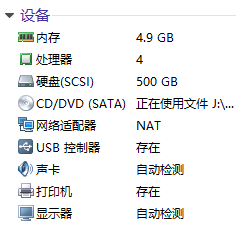
\includegraphics[width=0.6\textwidth]{./img/虚拟机设备配置.png}

    注意:\textbf{网络连接采取桥接(NAT)的方式进行连接}。

    ~

    安装完成之后的环境如下所示:

    ~

    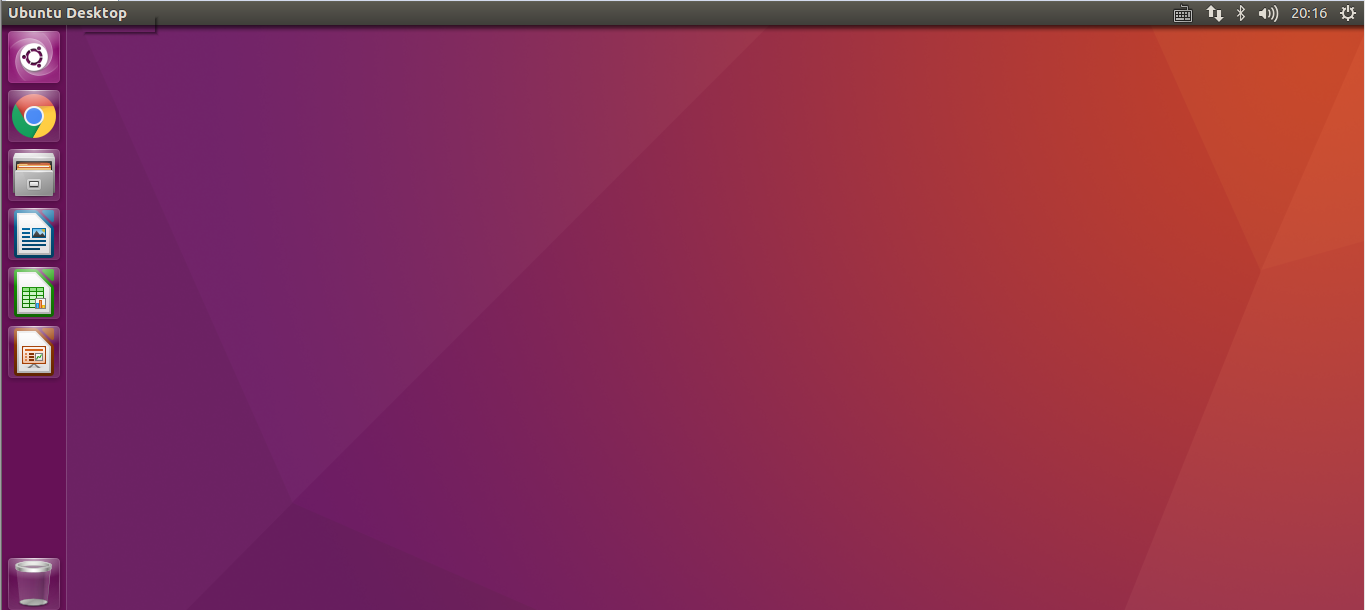
\includegraphics[width=0.8\textwidth]{./img/Ubuntu桌面图.png}

    \subsection{Step3: 开启vmware tools服务}
    VMware tools对于该项目的最大亮点是支持文件在虚拟机与物理机之间进行传输以及自动全屏扩展,因此其重要性不言而喻,之前使用过的centos系统,ubuntu gnome 16.04 都能够在虚拟机$--\>$ 设置 中点击VMware tools进行自动安装配置,而此处vmware tools由于是ubuntu lts 16.04或者其他缘故,因此需要手动安装。

    手动安装的过程如下:

    1. 使用$ctrl + alt + T$ 打开终端,再输入 $sudo su$切换到root模式;

    2. 将ISO挂载为CD-ROM,(测试机的ISO在$media/williamyi/VMware tools$): mount /media/williamyi/VMware tools /mnt/cdrom

    3. 用如下命令进行安装:

    \begin{lstlisting}[language=bash]
    cd /tmp
    tar -zxvf /mnt/cdrom/VMwareTools-<esx version>.i386.tar.gz
    \end{lstlisting}

    4. 运行VMware Tools安装程序。

        将目录更改到vmware-tools-distrib,然后运行./vmware-install.pl即可。

    5. 手动重启客户机(本人测试时关闭了物理机更改才生效)

    \subsection{Step4: 配置shadowsocks客户端}
    shadowsocks是啥,在此就不再进行解释了。此部分相对而言较为复杂,因为此前使用的代理均可以直接使用,而shadowsocks不太人性化,添加了许多额外的设置。其基本步骤如下:

    \paragraph{a. 使用命令行安装shadowsocks}

    ~

    \begin{lstlisting}[language=bash]
    apt-get install python-pip
    pip install shadowsocks
    \end{lstlisting}

    \paragraph{b. 创建启动配置文件shadowsocks.json}

    ~

    \begin{lstlisting}[language=bash]
    {
    "server":"***.***.***.***",
    "server_port":*****,
    "local_address": "127.0.0.1",
    "local_port":1080,
    "password":"******",
    "timeout":300,
    "method":"rc4-md5"
    }
    \end{lstlisting}

    其中,

    server 服务端的IP

    servier\_port 服务端的端口

    local\_port 本地端口,一般默认1080

    passwd ss服务端设置的密码

    timeout 超时设置 和服务端一样

    method 加密方法 和服务端一样


    \paragraph{c. 运行shadowsocks.json}

    ~

    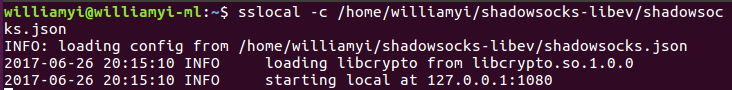
\includegraphics[width=1.0\textwidth]{./img/ss运行.png}

    上述完成的是全局代理的配置,以下为代理自动切换的配置:


    \paragraph{d. 下载SwitchyOmega插件}

    ~

    建议使用的是Chrome浏览器,同时给Chrome浏览器安装SwitchyOmega插件,关于其插件我们也可以在GitHub上直接下载(\url{https://github.com/FelisCatus/SwitchyOmega/releases/}), 然后浏览器地址打开\url{chrome://extensions/}, 将下载的插件进行安装即可。

    \paragraph{e. 配置浏览器插件}

    ~

    新建代理,取名为ss,配置如下:

    ~

    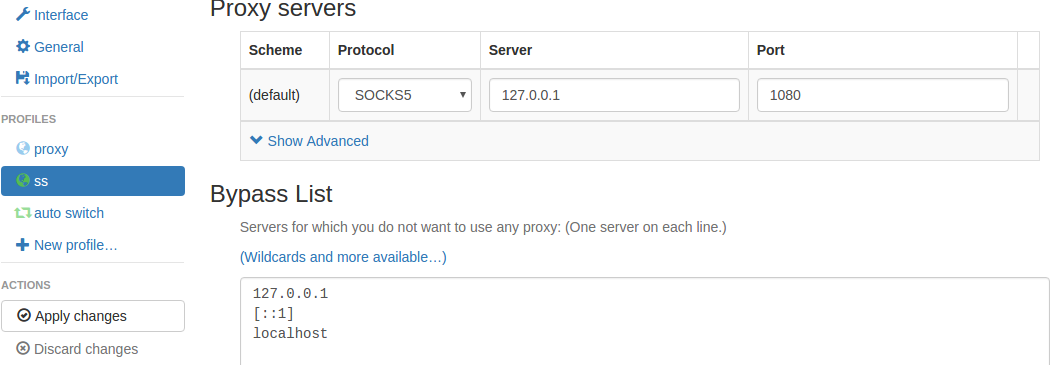
\includegraphics[width=1.0\textwidth]{./img/代理创建.png}

    ~

    然后点击到auto switch,进行代理选择配置:

    ~

    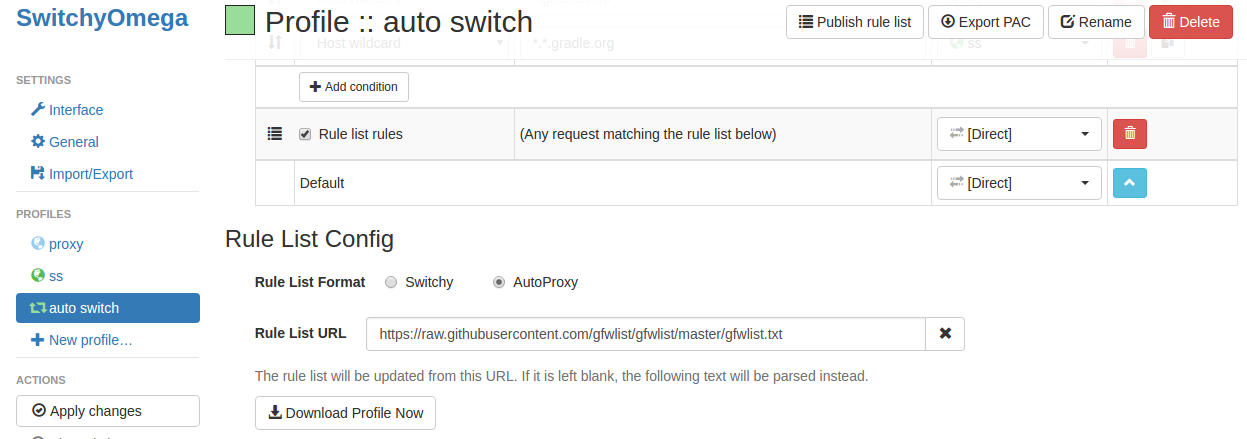
\includegraphics[width=1.0\textwidth]{./img/autoswitch配置.png}

    ~

    其中使用的rule list url 为:

    \url{https://raw.githubusercontent.com/gfwlist/gfwlist/master/gfwlist.txt}

    \paragraph{f. 代理运行}

    \begin{lstlisting}[language=bash]
    sslocal -c *.shadowsocks.json
    \end{lstlisting}

    至此大功告成。

    \section{Android Studio 与 Tensorflow平台配置}
    \subsection{Tensorflow平台搭建}
    tensorflow是谷歌公司开源的关于机器学习实践的平台,相关详细的介绍可以参考本人之前做的\href{https://github.com/WilliamYi96/Machine-Learning/blob/master/ML_Theories/Tensorflow/MNIST_for_ML_beginners%24Experts.md}{总结},  以及tensorflow\href{https://www.tensorflow.org/}{官方文档}。

    以下使用anaconda进行tensorflow的安装:

    \paragraph{a. 安装anaconda}

    ~

    按\href{https://www.continuum.io/downloads}{anaconda官网}介绍进行安装.

    \paragraph{b. 创建tensorflow的anaconda环境}

    \begin{lstlisting}[language=bash]
    $ conda create -n tensorflow
    \end{lstlisting}

    \paragraph{c. 激活anaconda环境}

    \begin{lstlisting}[language=bash]
    $ source activate tensorflow
    (tensorflow)$  # The prompt should change
    \end{lstlisting}

    \paragraph{d. 用命令行在环境之下下载tensorflow}

    \begin{lstlisting}[language=bash]
    (tensorflow)$ pip install --ignore-installed --upgrade \
    https://storage.googleapis.com/tensorflow/linux/cpu/ \
    tensorflow-1.2.0-cp36-cp36m-linux_x86_64.whl
    \end{lstlisting}

    此处下载的是CPU only的python3.6 tensorflow版本。

    创建完成,此后可以在该环境之下使用
    \begin{lstlisting}[language=bash]
    jupyter notebook
    \end{lstlisting}

    进行ipython的创作。

    \subsection{Android Studio平台搭建}
    \paragraph{a. 下载并安装android studio}

    ~

    在\href{https://developer.android.com/studio/index.html}{官网}上下载android studio。

    安装是傻瓜式安装,较为简单,在此不进行赘述。

    注: \textbf{目前在Ubuntu16.04中,环境变量自动配置完成,因此无需进行额外操作(如果有变化依变化为准)}

    \paragraph{b. ubuntu中启动android studio}

    ~

    android studio的启动路径为$~/android-studio/bin/$, 然后直接在命令行中运行$./studio.sh$即可。

    然后进行新工程的创建。

    此处android studio可能卡在了rebuilding **** 之上,导致这一问题的原因是gradle需要翻墙进行下载,方便的方式是我们先下载所需要的gradle,然后再在创建工程的$~/gradle/wrapper/gradle-wrapper.properties$中替换为如下文件内容:

    \begin{lstlisting}[language=bash]
    #Mon Jun 26 00:35:23 CST 2017
    distributionBase=GRADLE_USER_HOME
    distributionPath=wrapper/dists
    zipStoreBase=GRADLE_USER_HOME
    zipStorePath=wrapper/dists
    distributionUrl=gradle-3.3-all.zip
    \end{lstlisting}

    然后就可以很好的解决这个问题了。

    我们创建的项目名为DeepCamera, 并进行勾选C++ Support, android studio会自动下载ndk的部分文件,完整版在\href{https://developer.android.com/ndk/downloads/index.html}{官网}上获取。

    \subsection{AS与TF交互式平台搭建}
    \paragraph{a. 下载tensorflow源码}

    \begin{lstlisting}[language=bash]
    git clone --recurse-submodules  \
    https://github.com/tensorflow/tensorflow.git
    \end{lstlisting}

    \paragraph{b. WORKSPACE 文件修改}

    ~

    打开tensorflow文件夹下的WORKSPACE, 部分原文件为

    \begin{lstlisting}[language=bash]
    # Uncomment and update the paths in these entries
    # to build the Android demo.
    #android_sdk_repository(
    #    name = "androidsdk",
    #    api_level = 23,
    #    build_tools_version = "25.0.1",
    #    # Replace with path to Android SDK on your system
    #    path = "<PATH_TO_SDK>",
    #)
    #
    #android_ndk_repository(
    #    name="androidndk",
    #    path="<PATH_TO_NDK>",
    #    api_level=14)
    \end{lstlisting}

    修改为:

    \begin{lstlisting}[language=bash]
    # Uncomment and update the paths in these entries
    # to build the Android demo.
    android_sdk_repository(
    name = "androidsdk",
    api_level = 26,
    # Ensure that you have the build_tools_version
        below installed in the
    # SDK manager as it updates periodically.
    build_tools_version = "26.0.0",
    # Replace with path to Android SDK on your system
    path = "/home/williamyi/Android/Sdk",
    )

    # Android NDK r12b is recommended
        (higher may cause issues with Bazel)
    android_ndk_repository(
    name = "androidndk",
    path = "/home/williamyi/Android/Ndk/android-ndk-r12b",
    # This needs to be 14 or higher to compile TensorFlow.
    # Note that the NDK version is not the API level.
    api_level = 26)
    \end{lstlisting}

    \paragraph{c. 编译得到.so文件}

    \begin{lstlisting}[language=bash]
    bazel build -c opt //tensorflow/contrib/android:libtensorflow_inference.so \
       --crosstool_top=//external:android/crosstool \
       --host_crosstool_top=@bazel_tools//tools/cpp:toolchain \
       --cpu=armeabi-v7a
    \end{lstlisting}

    运行情况如下:

    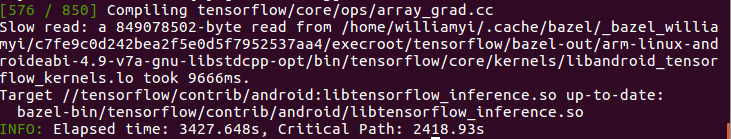
\includegraphics[width=1.0\textwidth]{img/TensorFlow编译.png}

    该文件将在如下位置处找到:

    \begin{lstlisting}[language=bash]
    bazel-bin/tensorflow/contrib/android/libtensorflow_inference.so
    \end{lstlisting}

    \paragraph{d. 编译得到.jar文件}

    \begin{lstlisting}[language=bash]
    bazel-bin/tensorflow/contrib/android/libtensorflow_inference.so
    \end{lstlisting}

    运行情况如下:

    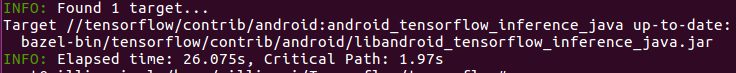
\includegraphics[width=1.0\textwidth]{img/TensorFlow-java编译.png}

    该文件将在如下位置找到:

    \begin{lstlisting}[language=bash]
    bazel-bin/tensorflow/contrib/android/libtensorflow_inference.so
    \end{lstlisting}

    注:\textbf{在编译过程中报错的诸多问题发现都是WORKSPACE更改不恰当,比如ndk路径不正确,没有使用r12b,使用版本不正确等,注意反复检查WORKSPACE}

    \chapter{项目测试}
    \section{测试总体情况}
    \begin{table}[!htb]
      \centering
      \begin{tabular}{|c|c|c|}
        \hline
        % after \\: \hline or \cline{col1-col2} \cline{col3-col4} ...
        模块功能 & 情况 & 备注 \\
        \textbf{欢迎界面}\\
        Welcome开机运行 & 成功  & 通过 \\
        Welcome两秒后跳转至MainActivity & 成功 & 通过 \\
        \textbf{主界面}& \\
        Camera显示 & 成功 & 通过 \\
        切换相机 & 前后镜切换 & 通过 \\
        探测物体 & 拍摄照片并显示 & 通过 \\
        点击Backup后Toast Backup & Toast Backup & 通过 \\
        点击Delete后Toast Delete & Toast Delete & 通过 \\
        点击Settings后Toast Settings & Toast Settings & 通过\\
        \textbf{个人简历} & \\
        简历界面显示 & 成功 & 通过\\
        Back键 & 返回到Camera & 通过\\
        English键 & 点击转换为英文 & 通过 \\
        Github键 & 在当前应用打开个人GitHub & 通过 \\
        Project键 & 打开本项目网站 & 通过 \\
        Weibo键 & 打开个人微博 & 通过\\
        \textbf{Personal Info} & \\
        简历英文显示 & 成功 & 通过 \\
        Back键 & 返回到Camera & 通过\\
        中文键 & 点击转换为中文 & 通过\\
        Github键 & 在当前应用打开个人GitHub & 通过 \\
        Project键 & 打开本项目网站 & 通过 \\
        Weibo键 & 打开个人微博 & 通过\\
        \textbf{通过率} & 100\% \\
        \hline
      \end{tabular}
      \caption{测试总体情况}\label{测试总体情况}
    \end{table}
    \section{基础显示测试}
    \subsection{欢迎界面-主界面}
    \begin{figure}[!htb]
    \centering
    \begin{minipage}[c]{0.5\textwidth}
    \centering
    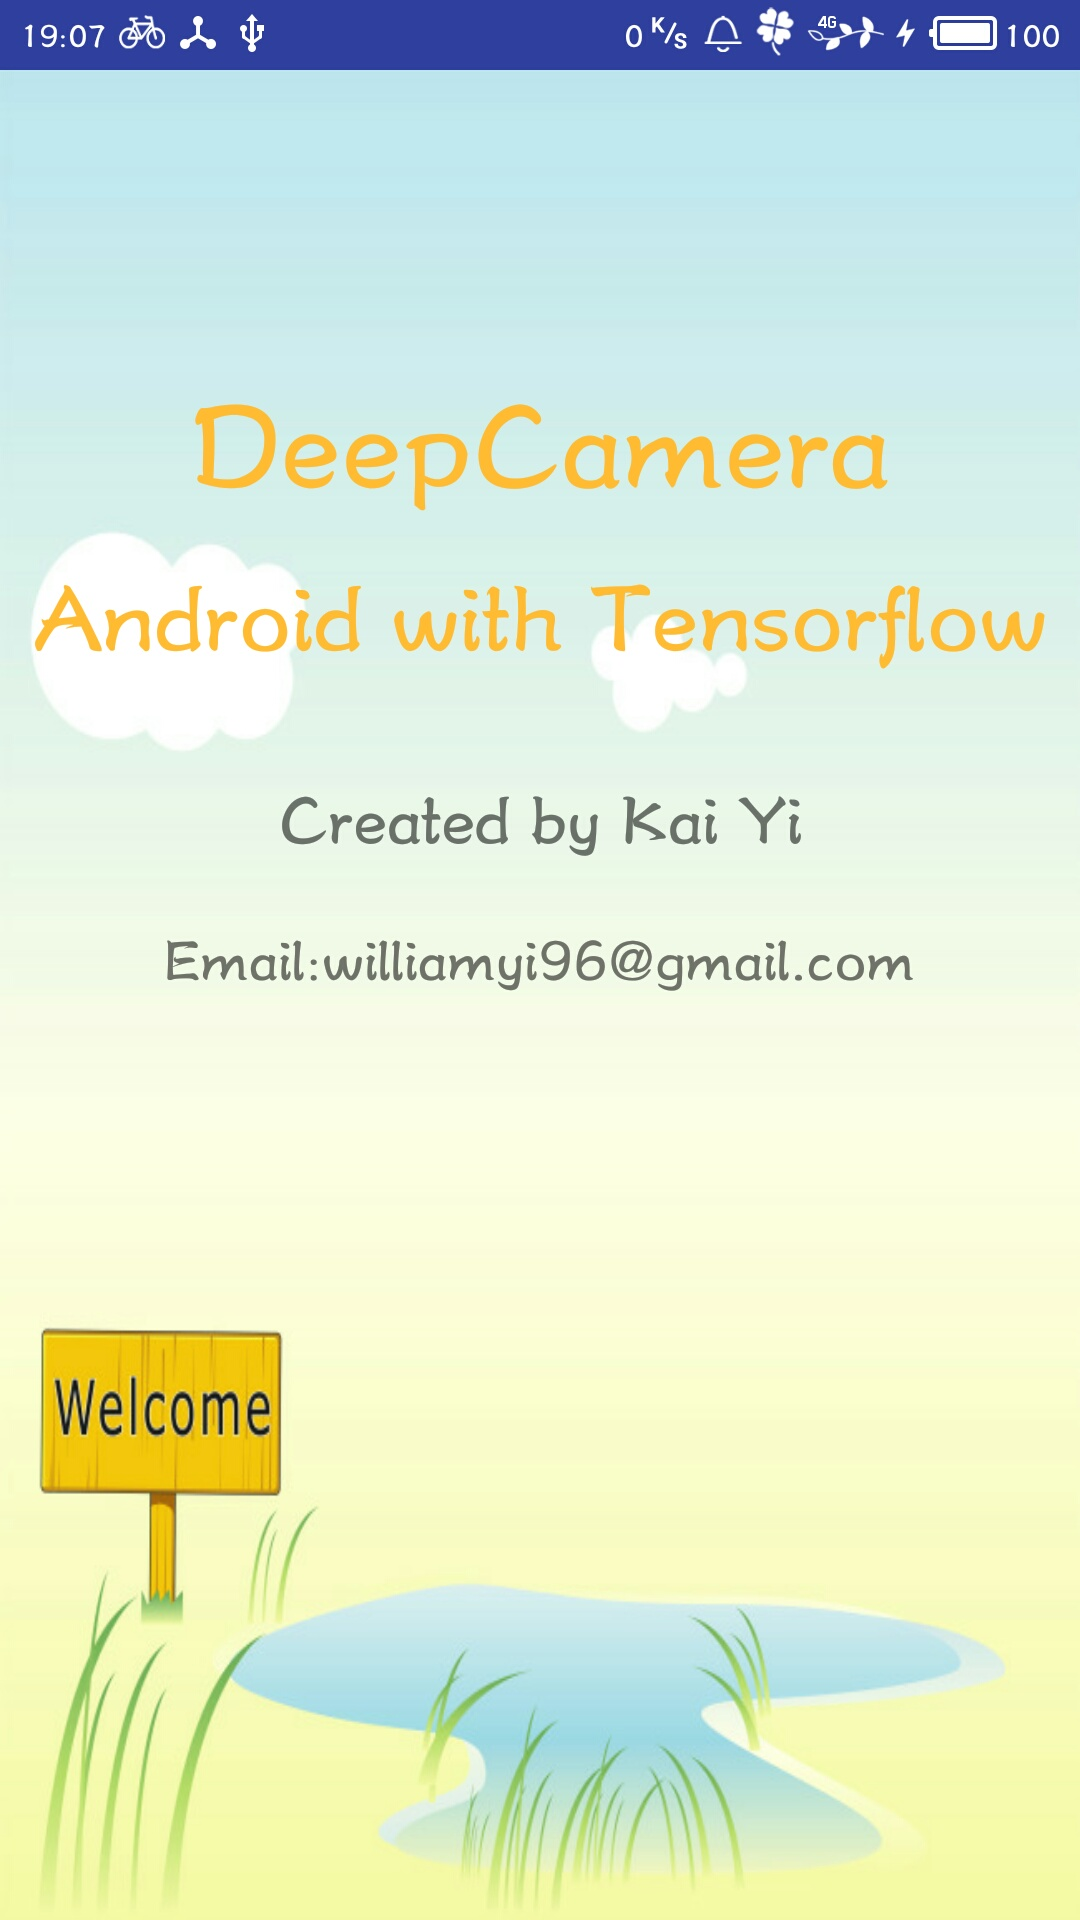
\includegraphics[width=0.92\textwidth]{img/欢迎界面.png}
    \end{minipage}%
    \begin{minipage}[c]{0.5\textwidth}
    \centering
    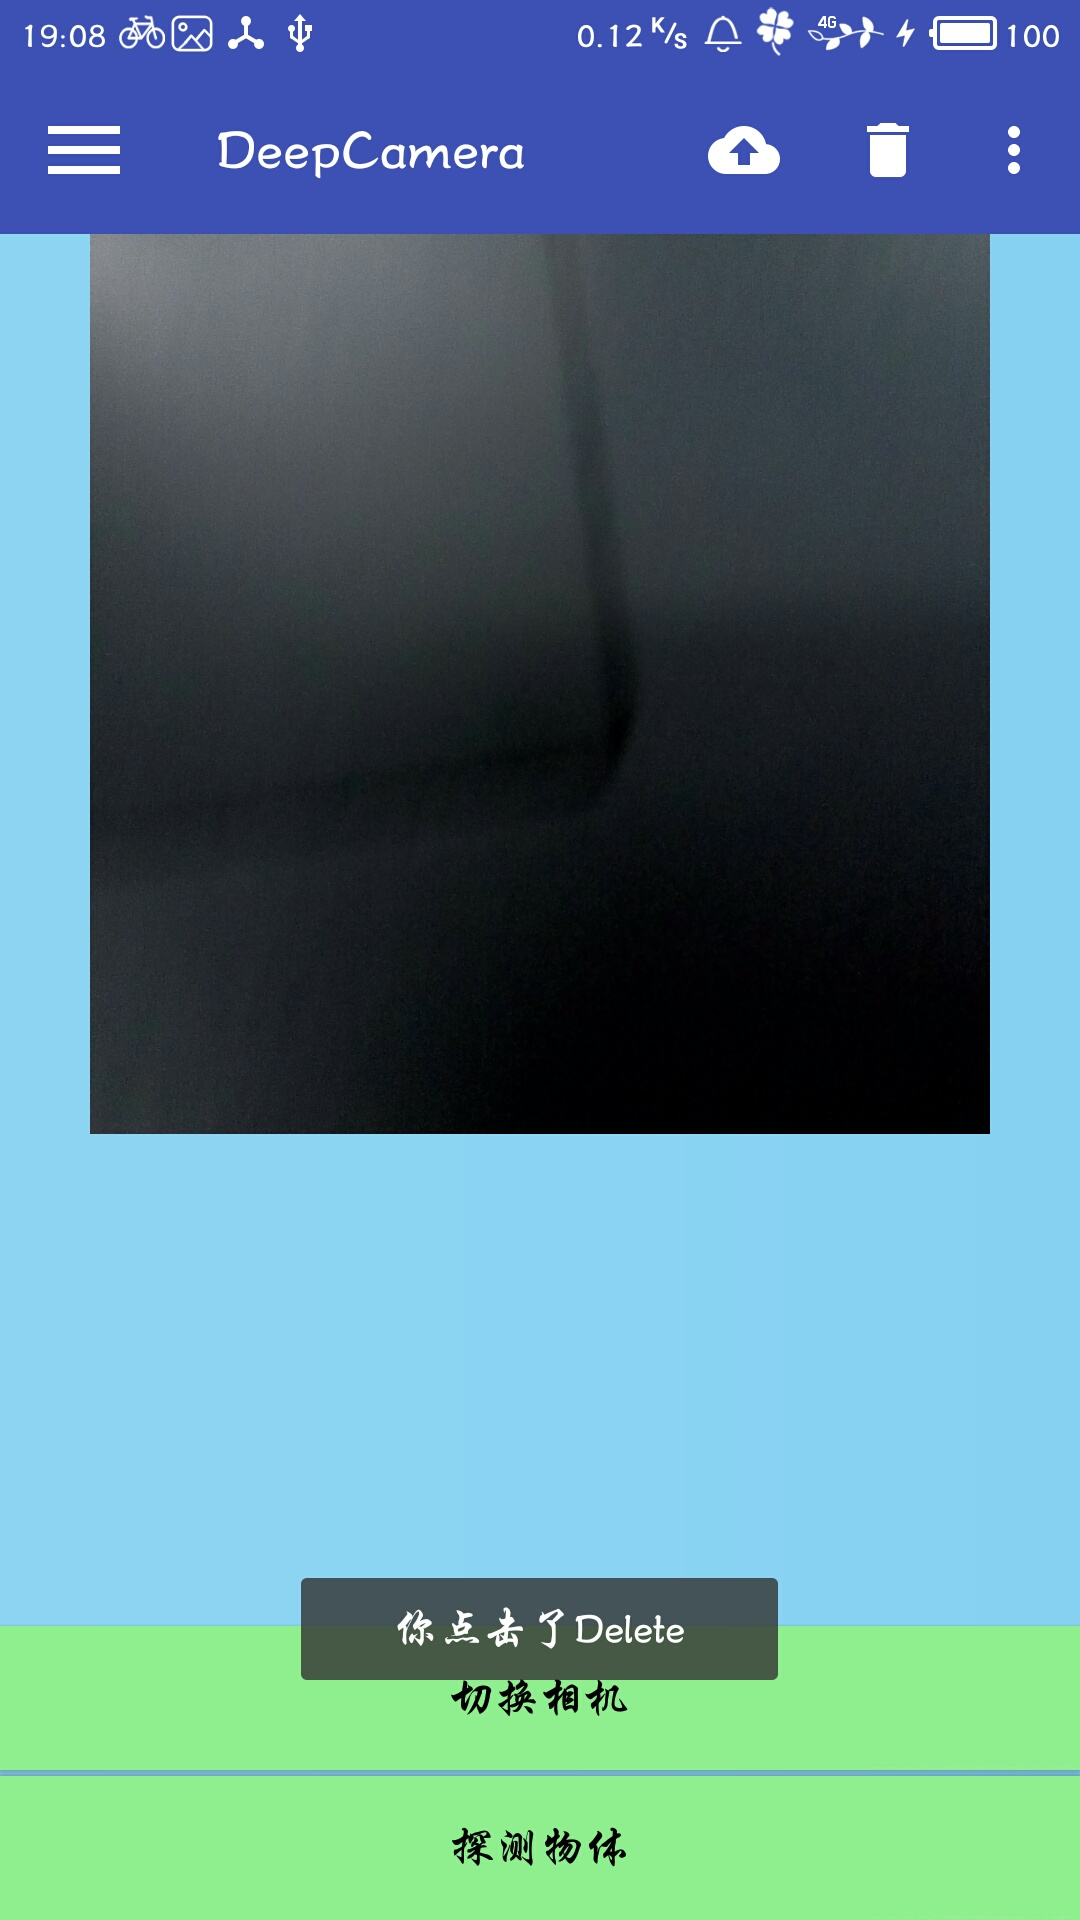
\includegraphics[width=0.92\textwidth]{img/主界面.png}
    \end{minipage}
    \caption{欢迎界面-主界面}
    \end{figure}

    \subsection{个人简历-Personal Info}
    \begin{figure}[!htb]
    \centering
    \begin{minipage}[c]{0.5\textwidth}
    \centering
    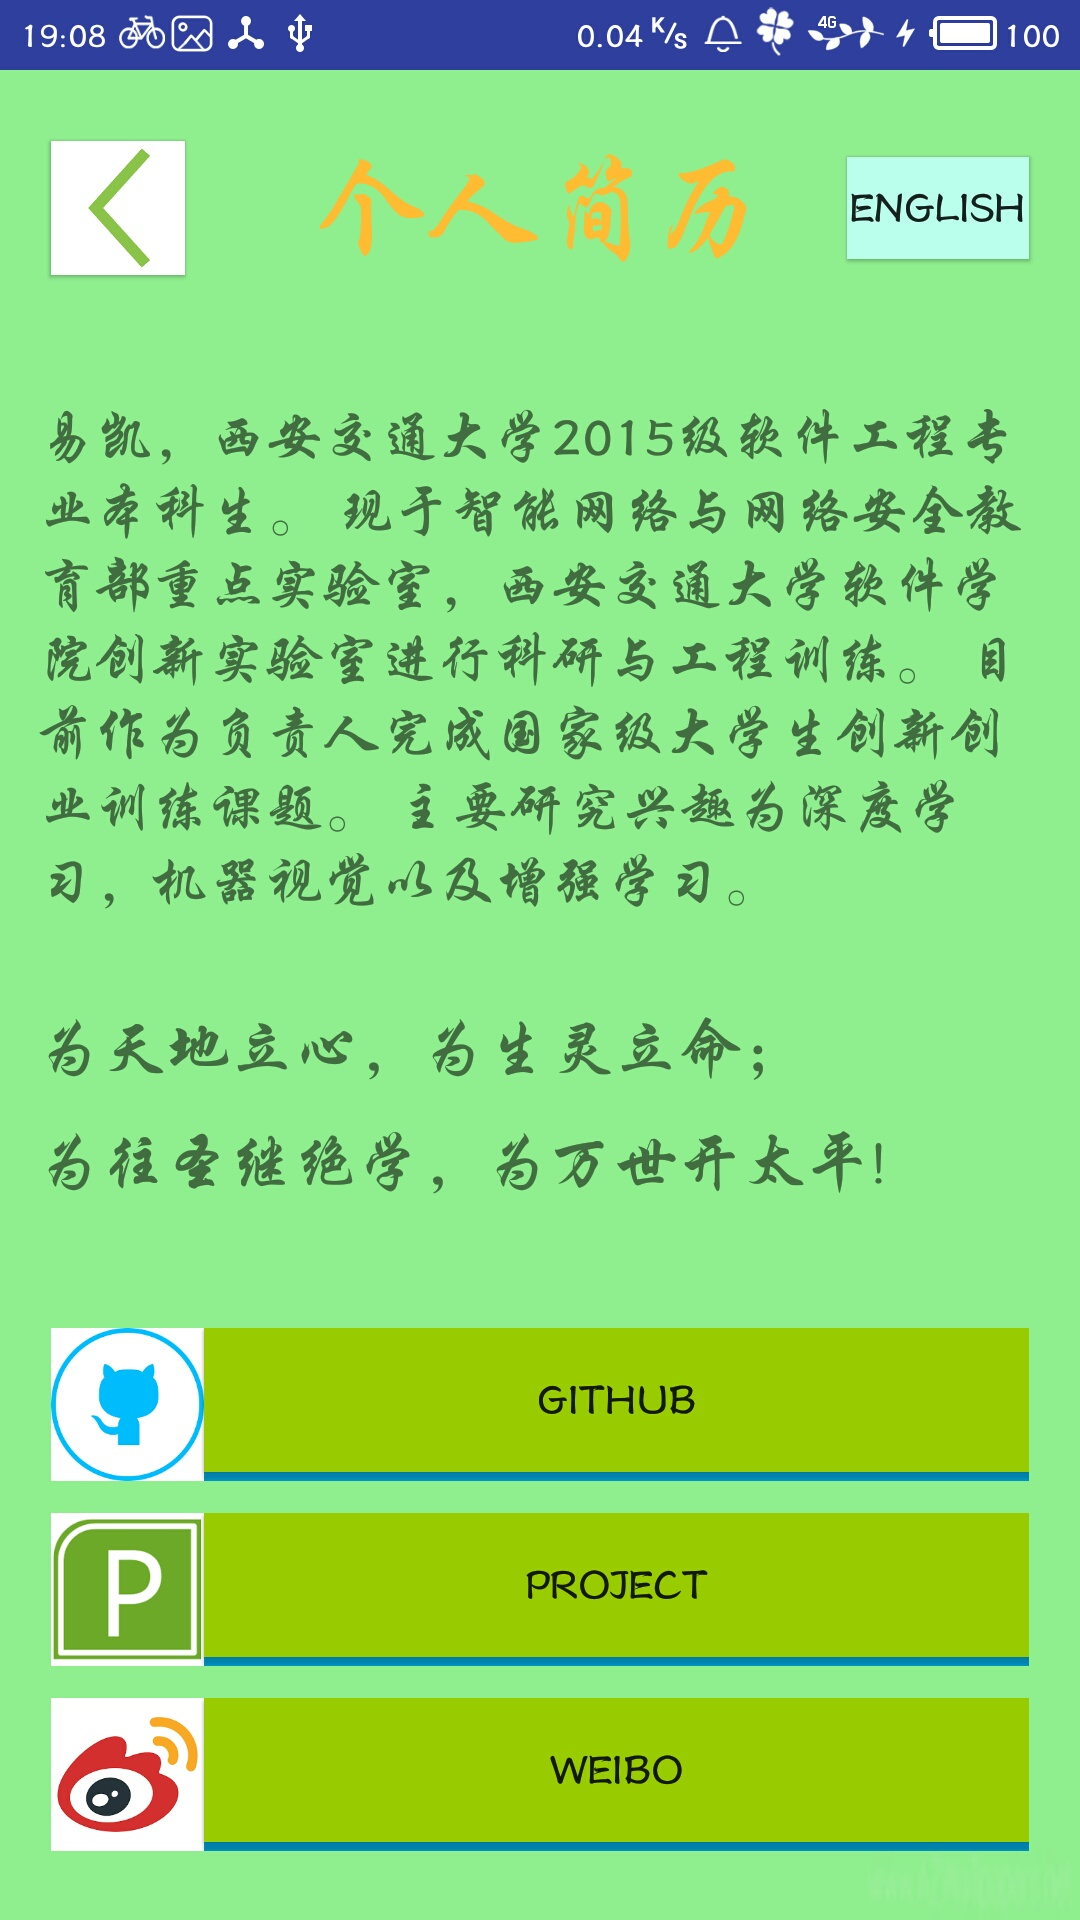
\includegraphics[width=0.92\textwidth]{img/个人简历界面.png}
    \end{minipage}%
    \begin{minipage}[c]{0.5\textwidth}
    \centering
    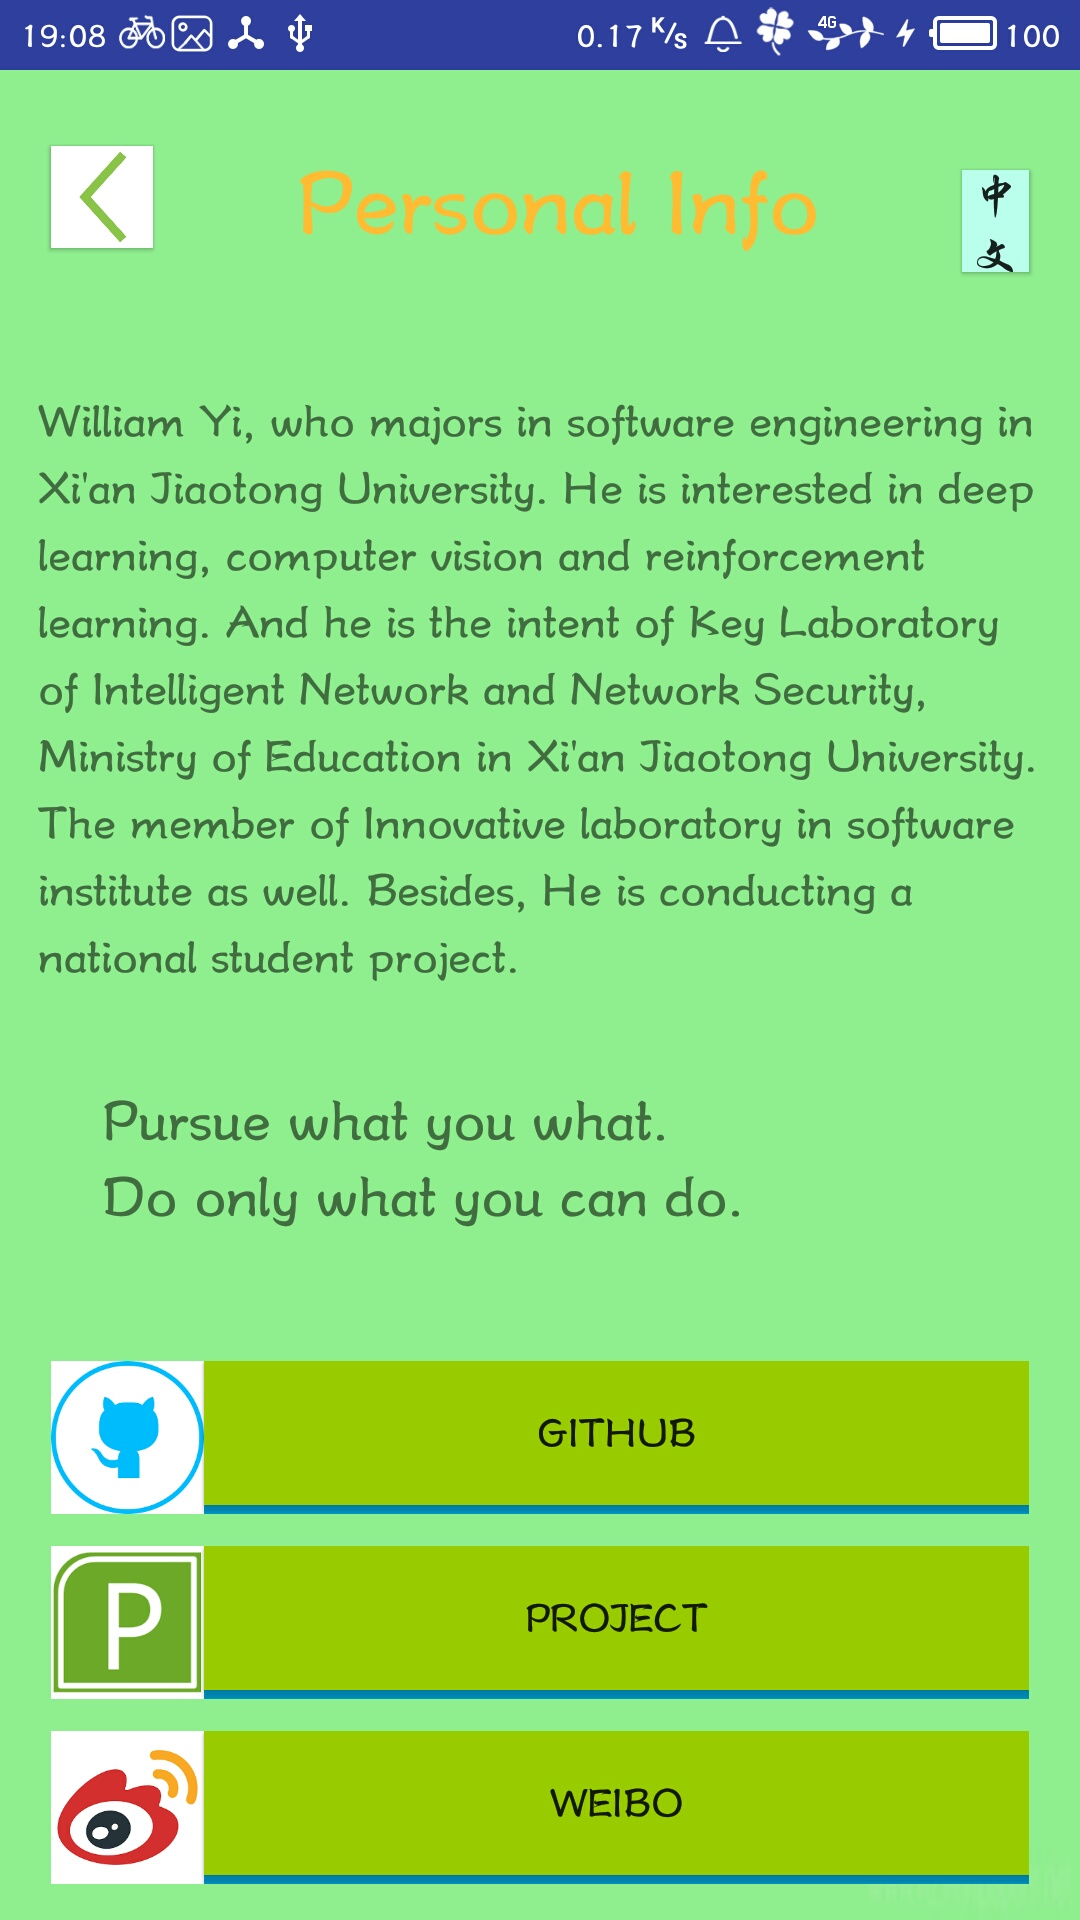
\includegraphics[width=0.92\textwidth]{img/PersonalInfo.png}
    \end{minipage}
    \caption{欢迎界面-主界面}
    \end{figure}

    \subsection{跳转界面-Github-Project-Weibo}
    \begin{figure}[!htb]
    \centering
    \begin{minipage}[c]{0.33\textwidth}
    \centering
    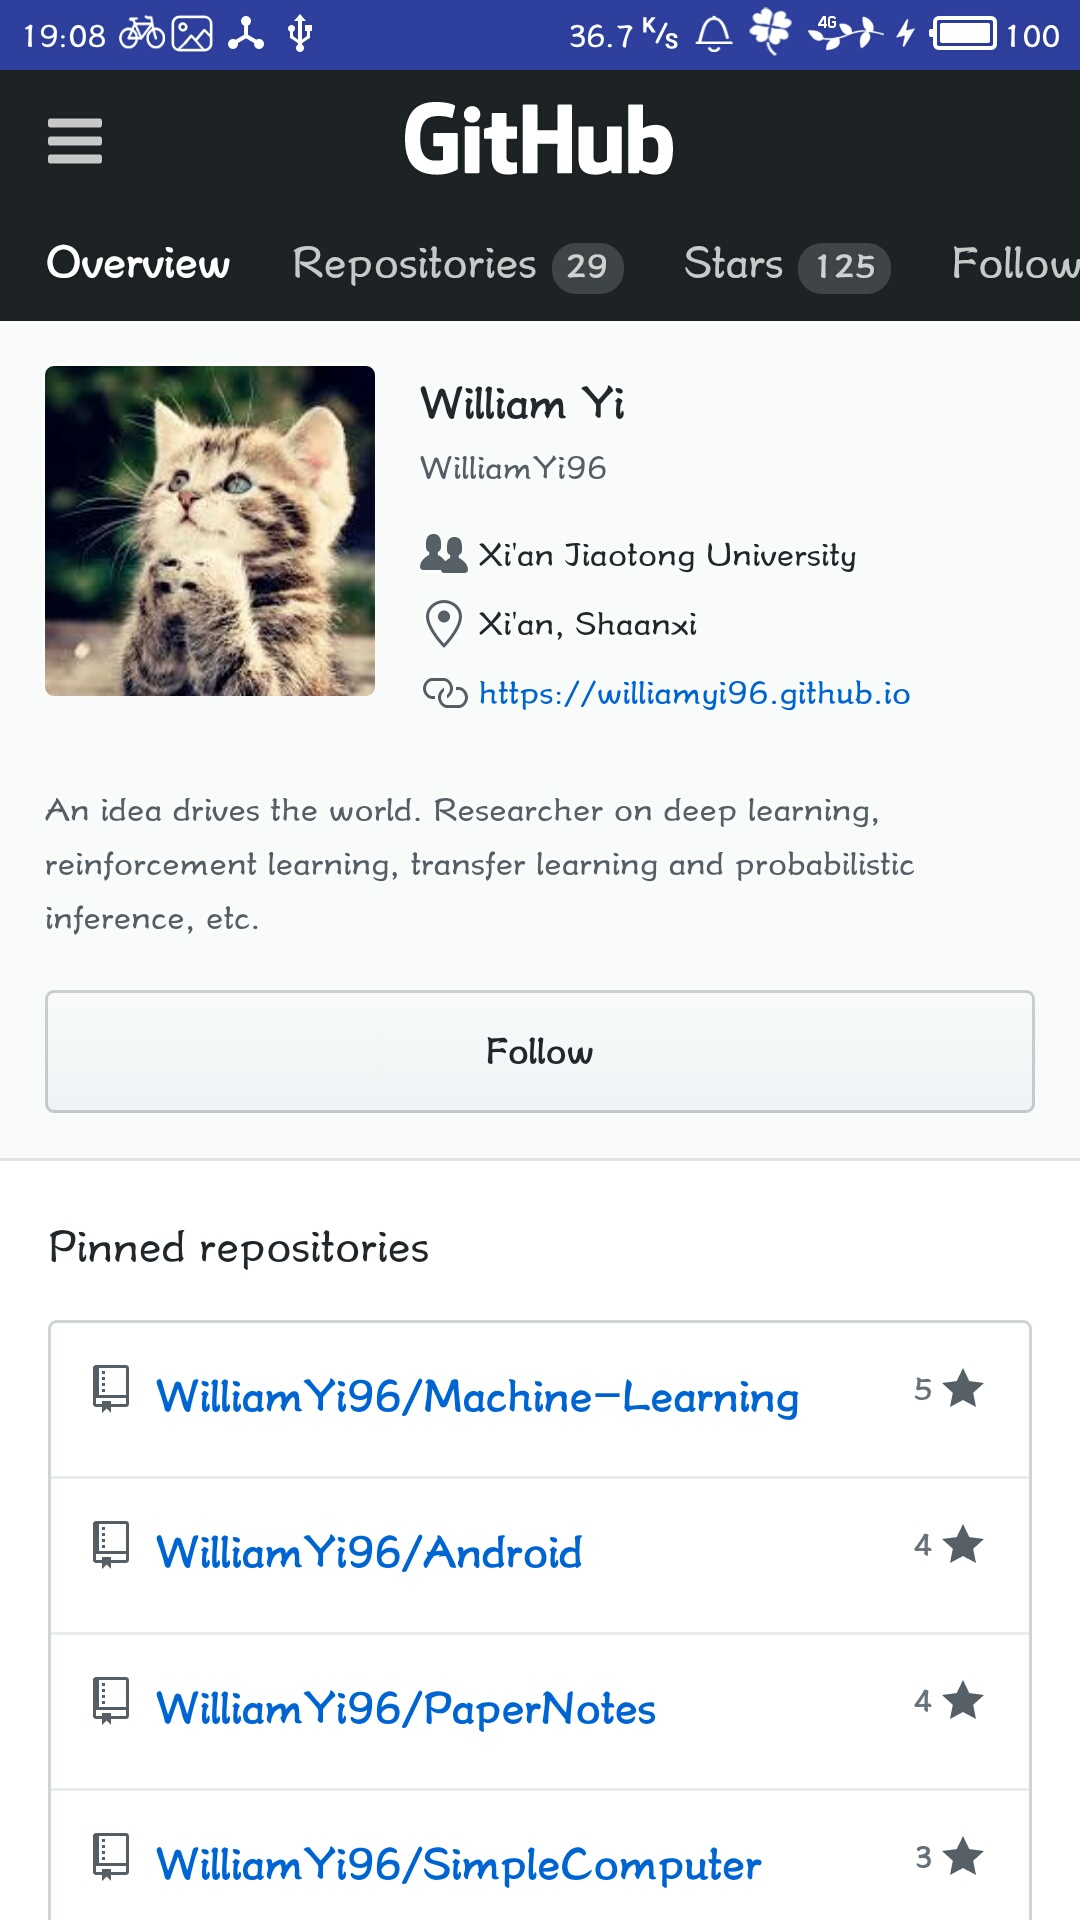
\includegraphics[width=0.92\textwidth]{img/github.png}
    \end{minipage}%
    \begin{minipage}[c]{0.33\textwidth}
    \centering
    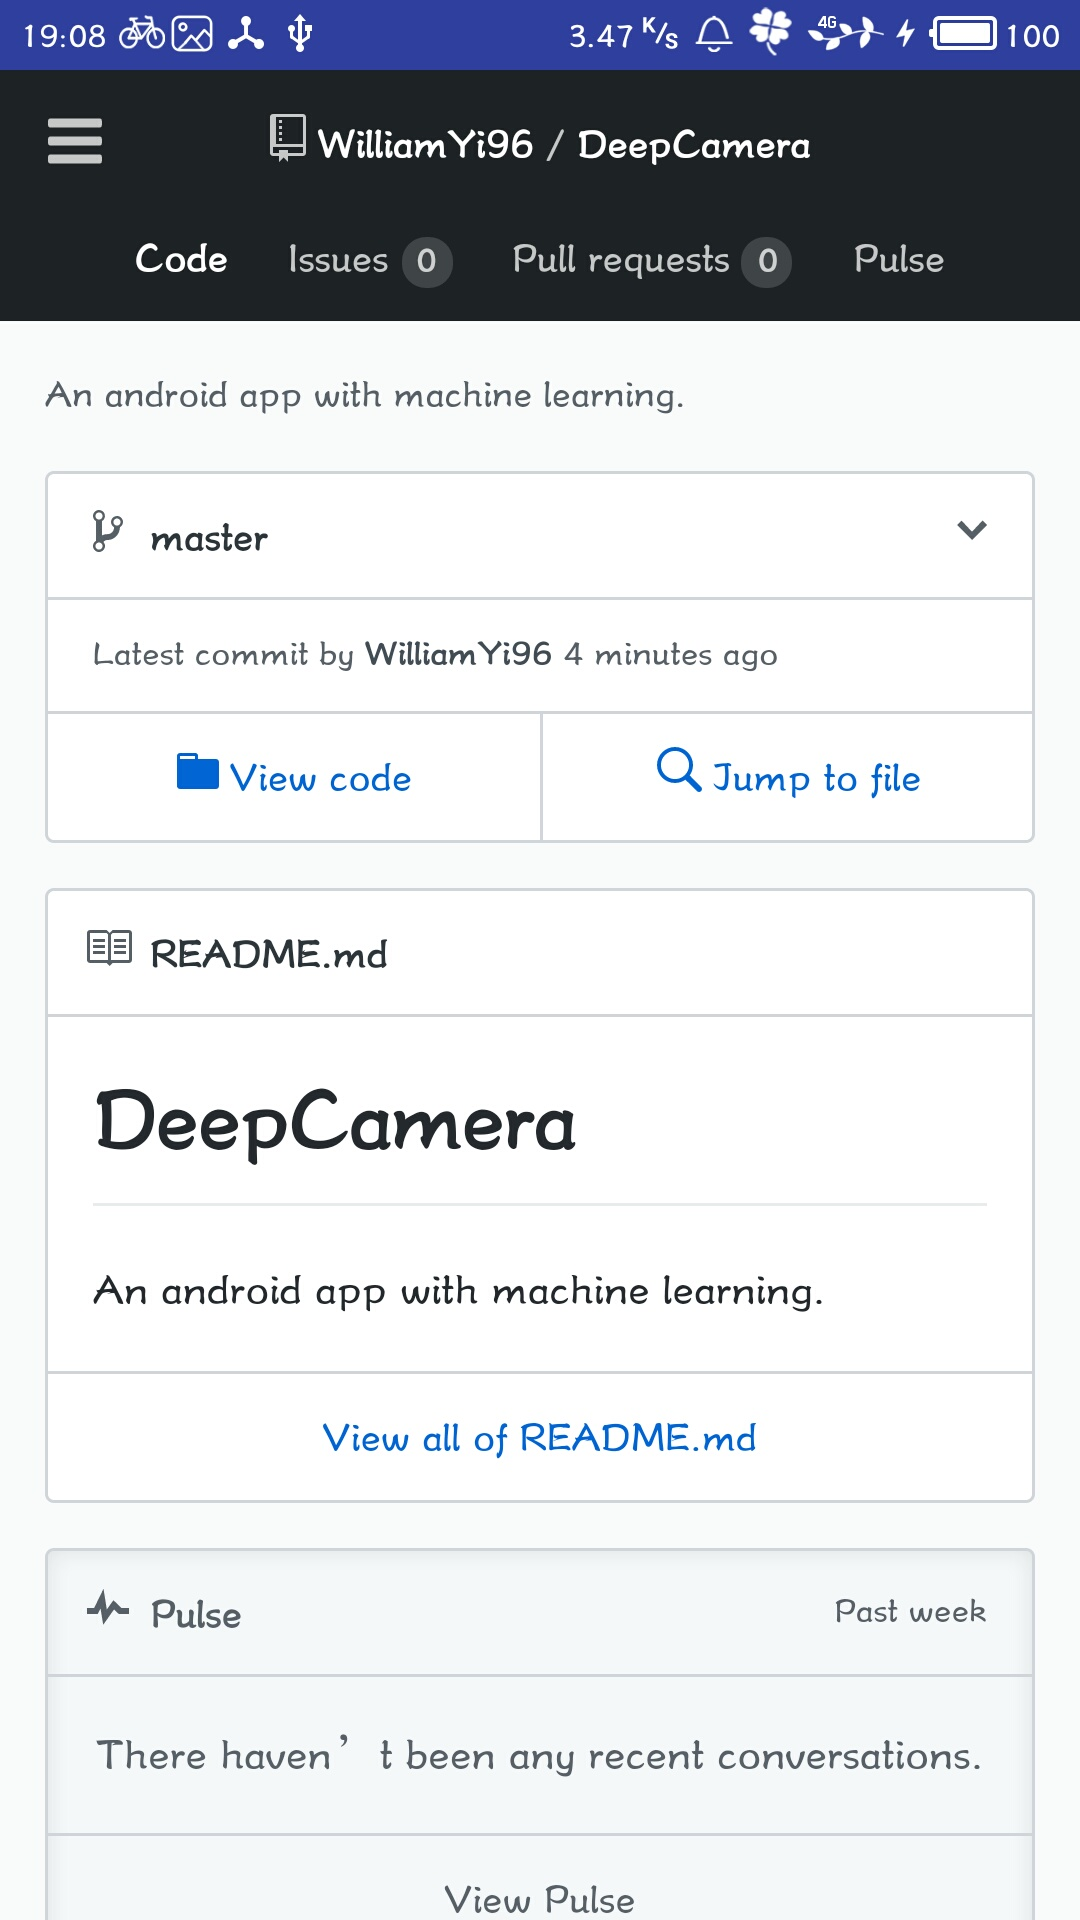
\includegraphics[width=0.92\textwidth]{img/project.png}
    \end{minipage}
    \begin{minipage}[c]{0.33\textwidth}
    \centering
     
\includegraphics[width=0.92\textwidth]{img/weibo.png}
    \end{minipage}
    \caption{跳转界面}
    \end{figure}

    \section{相机运行测试}
    \begin{figure}[!htb]
    \centering
    \begin{minipage}[c]{0.5\textwidth}
    \centering
    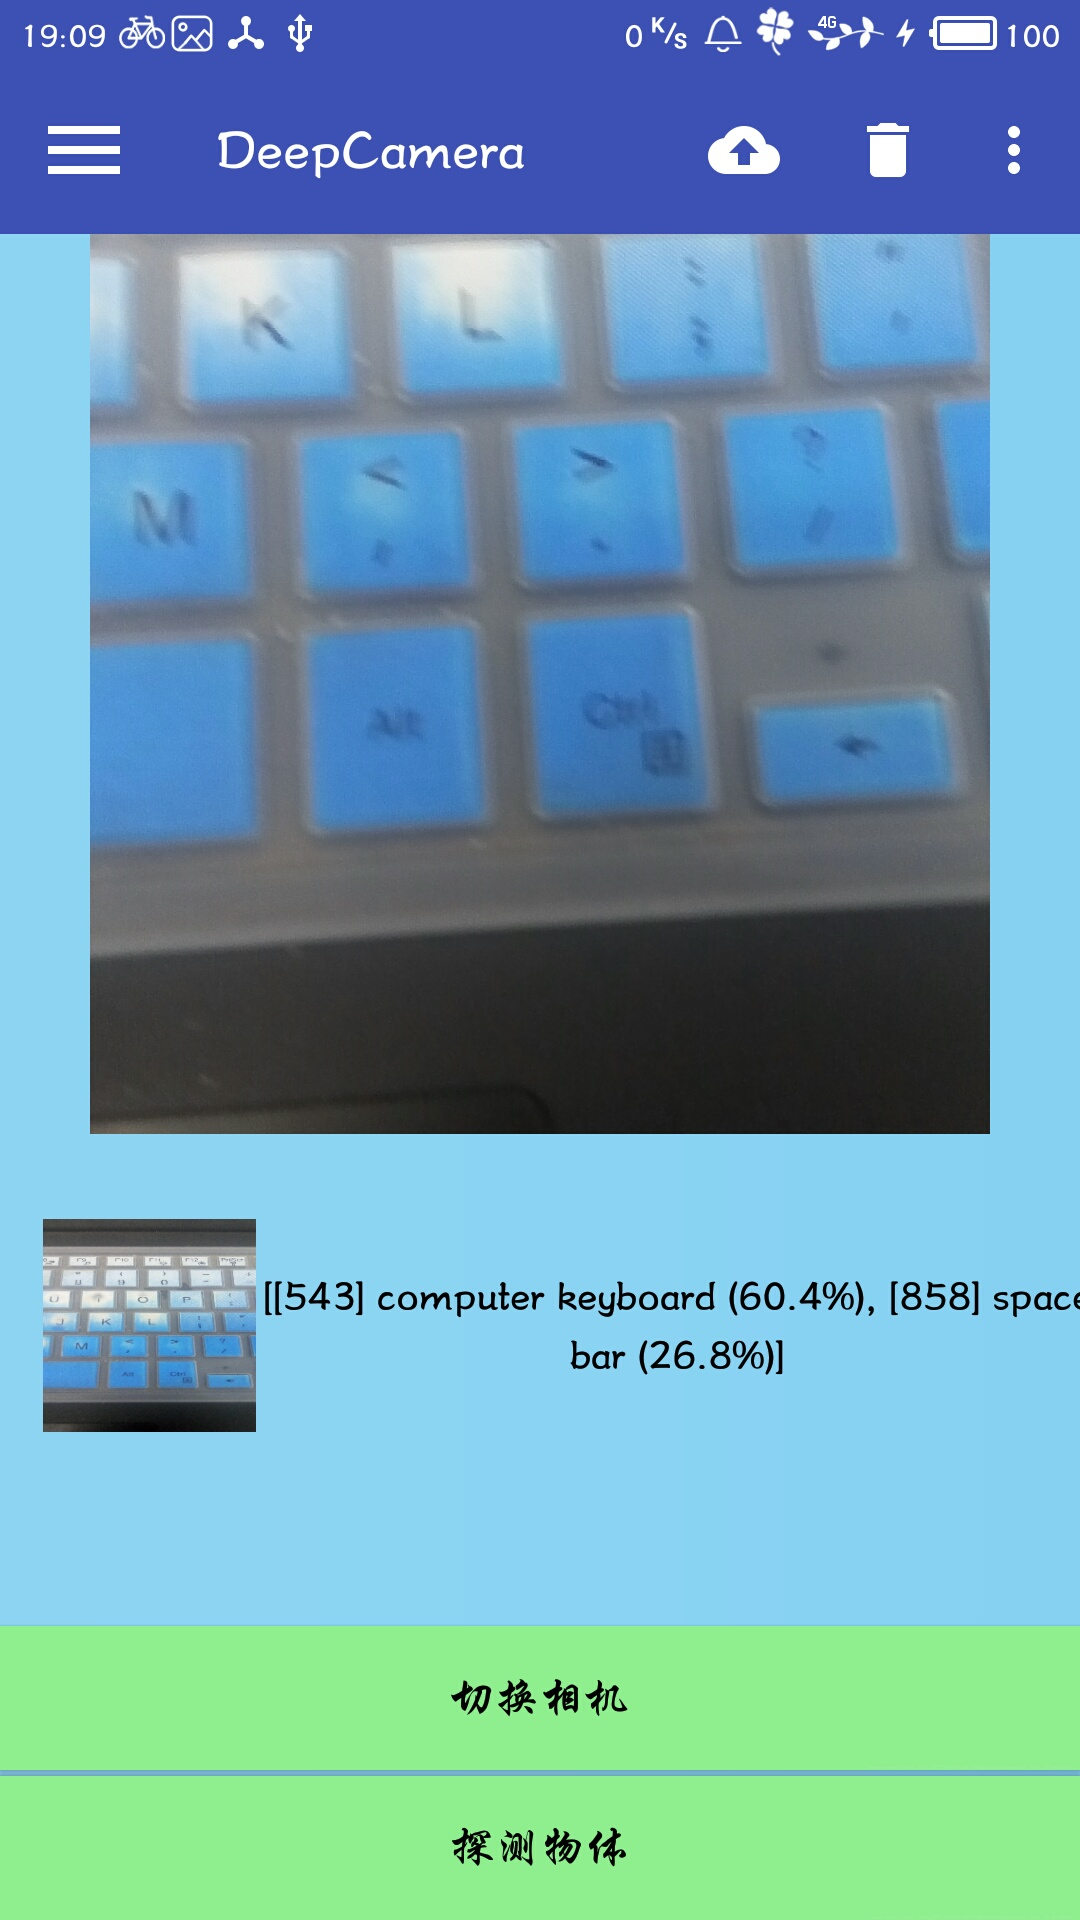
\includegraphics[width=0.92\textwidth]{img/test1.png}
    \end{minipage}%
    \begin{minipage}[c]{0.5\textwidth}
    \centering
    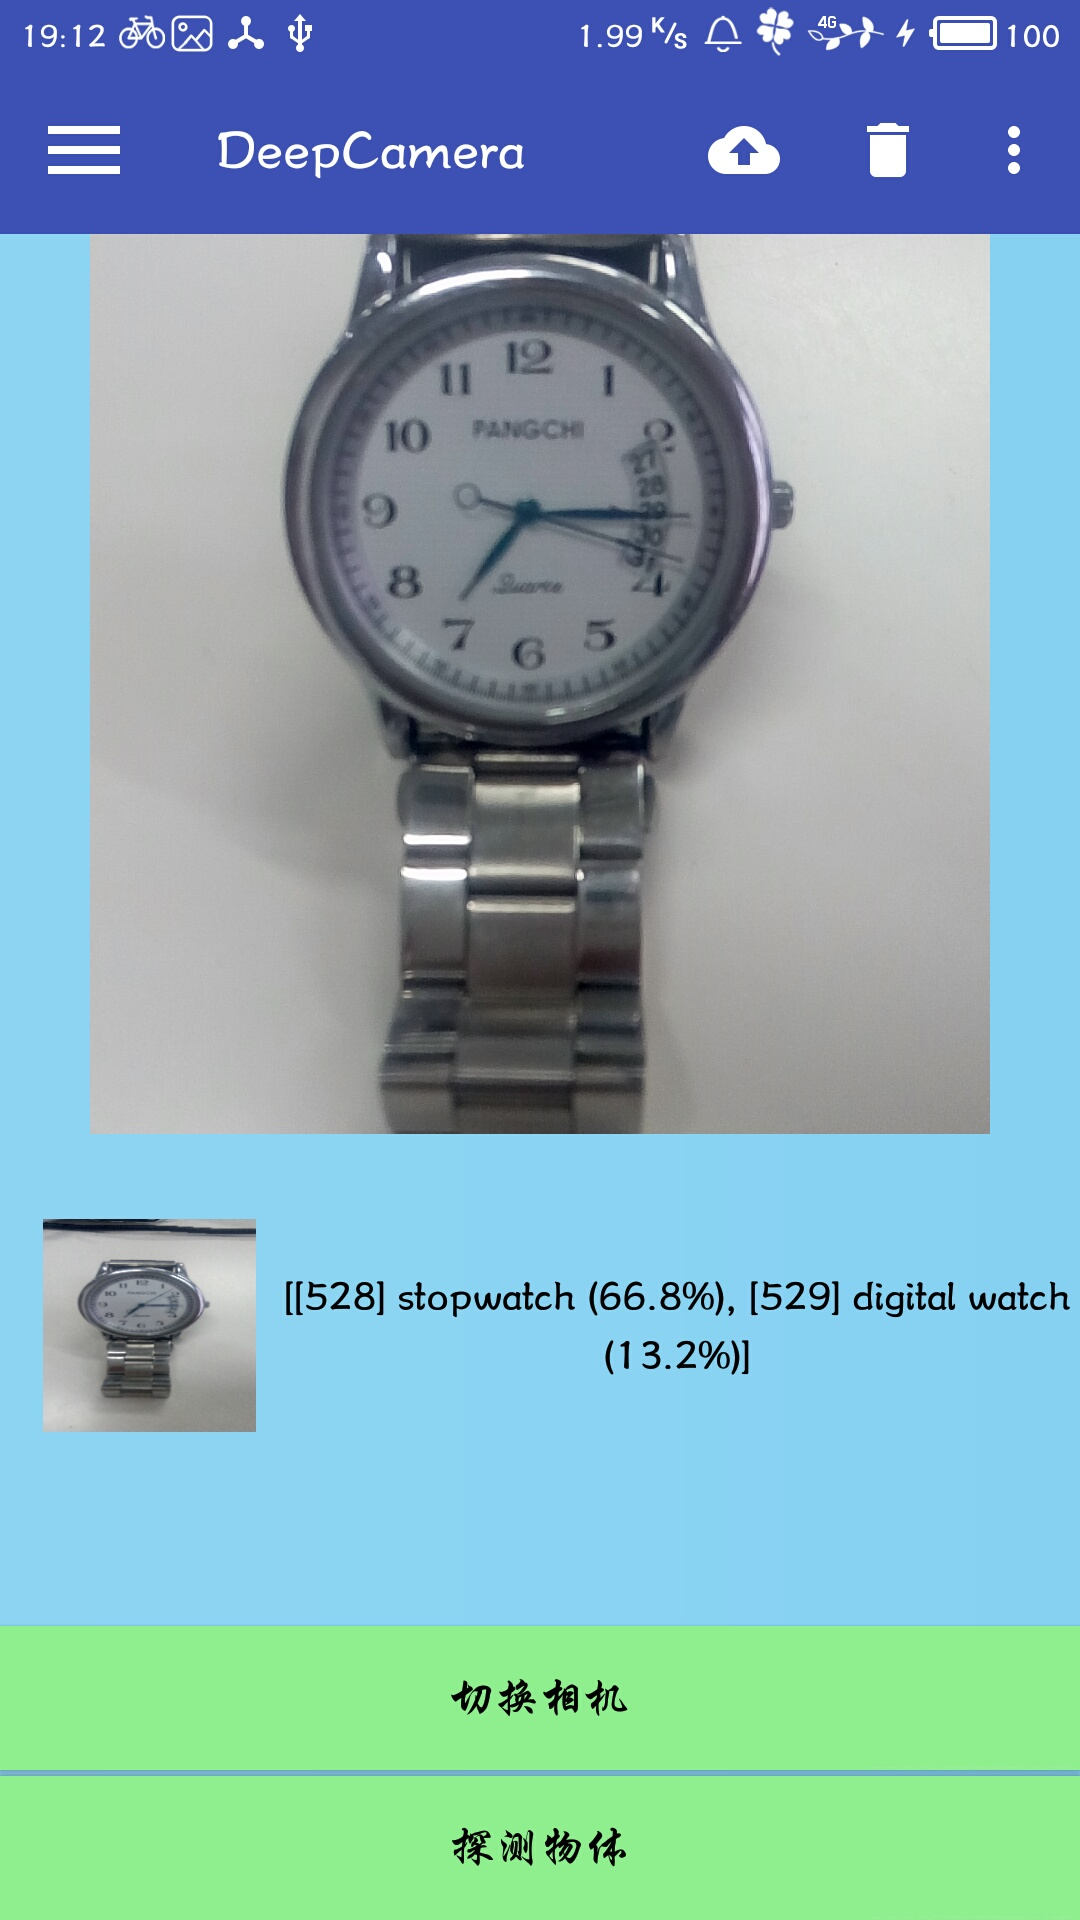
\includegraphics[width=0.92\textwidth]{img/test2.png}
    \end{minipage}
    \caption{相机运行测试结果1}
    \end{figure}

    \begin{figure}[!htb]
    \centering
    \begin{minipage}[c]{0.33\textwidth}
    \centering
    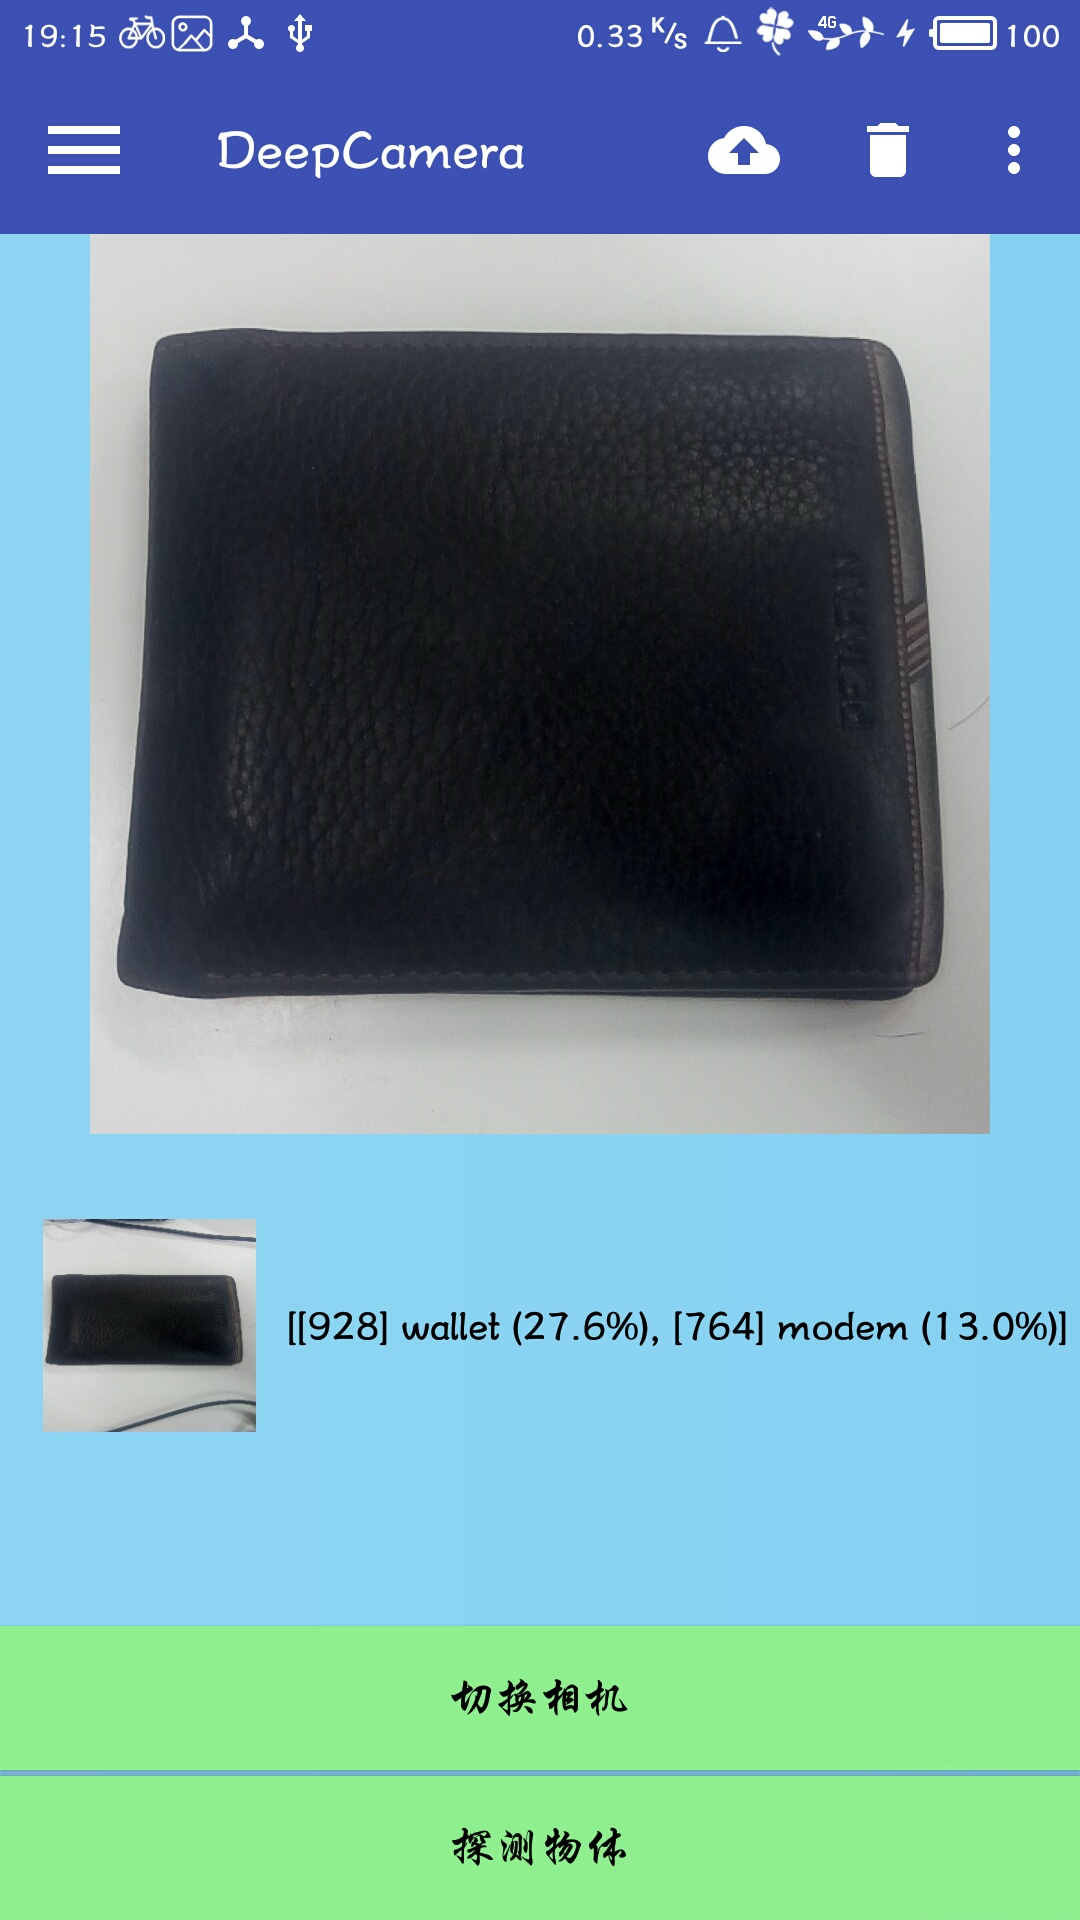
\includegraphics[width=0.92\textwidth]{img/test3.png}
    \end{minipage}%
    \begin{minipage}[c]{0.33\textwidth}
    \centering
    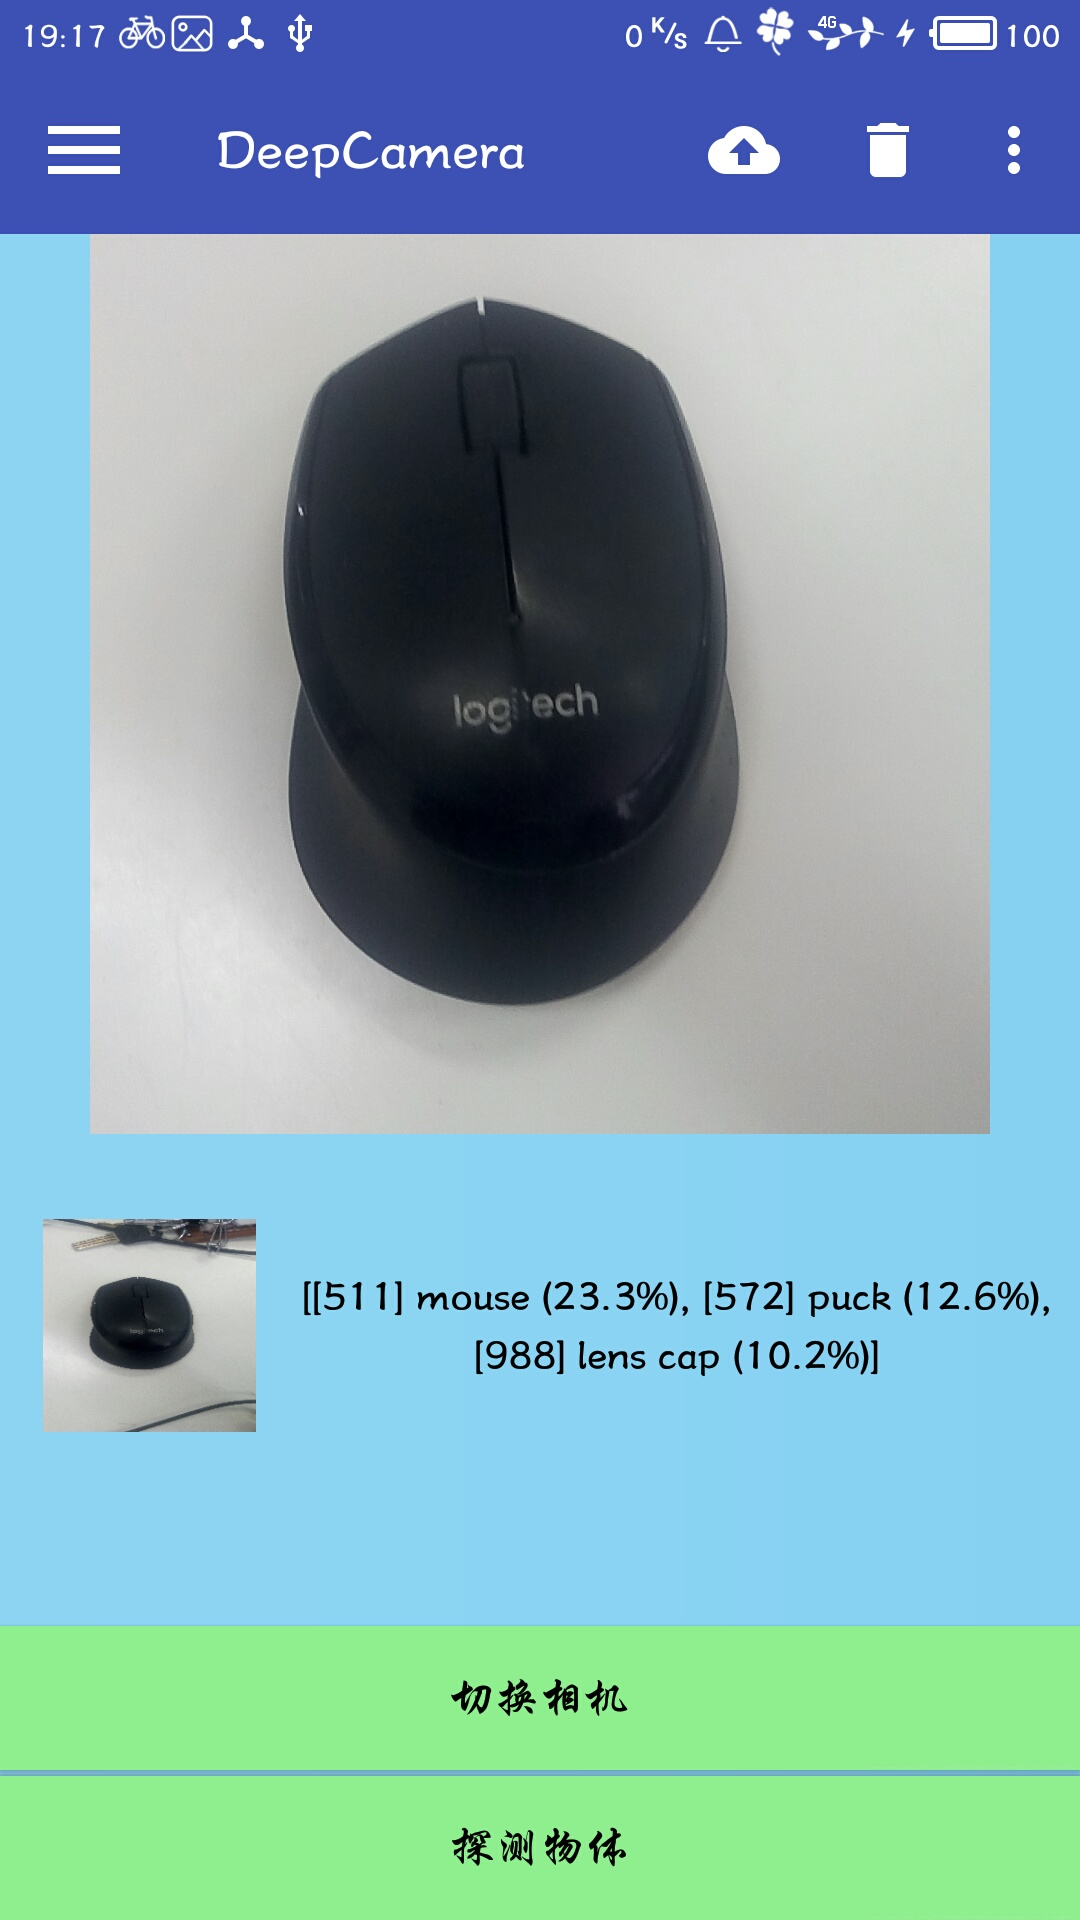
\includegraphics[width=0.92\textwidth]{img/test4.png}  
    \end{minipage}
    \begin{minipage}[c]{0.33\textwidth}
    \centering
    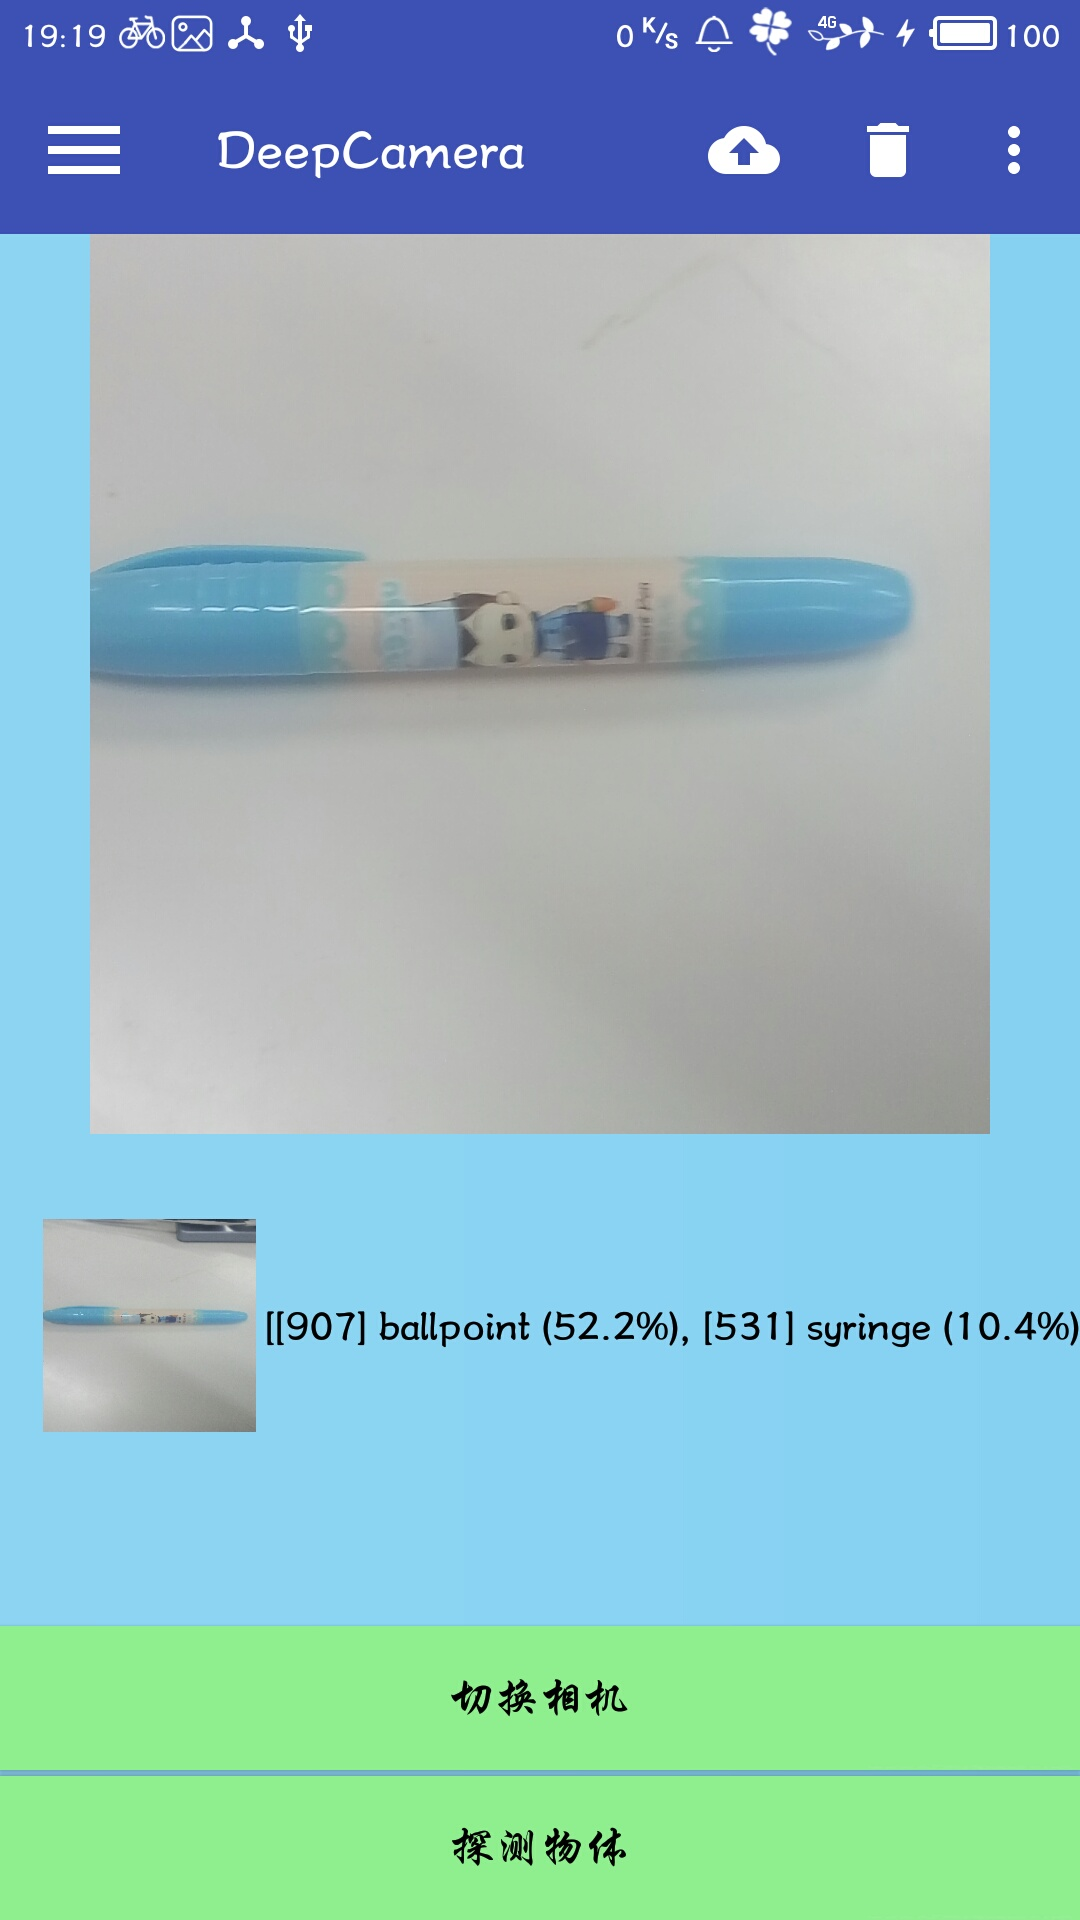
\includegraphics[width=0.92\textwidth]{img/test5.png}
    \end{minipage}
    \caption{相机运行测试结果2}
    \end{figure}

    \chapter{实验总结}
    \section{基本介绍}
    为时一个学期的《嵌入式软件设计》课程的学习就这样结束了,这一路走来,受益良多。通过嵌入式软件以及安卓应用开发的学习,对于相关知识有了较为深入的理解。在大作业是选择嵌入式软件设计还是安卓应用开发的节骨眼上,起初我选择了嵌入式软件设计,原本想借此机会对于计算机有一个深入的理解,慢慢发现底层的东西理解难度是一方面,另外一方面,遇到了有些错误竟然也不知道如何去解决,后来忍痛选择了安卓应用开发。但是为了将两者贴合起来,因此我决定初次使用ndk进行程序设计。

    由于本人目标是成为一名出色的机器学习科学家,因此想要尝试在保留安卓基础程序设计的框架基础上,将机器学习应用于安卓程序设计来写一个程序,由此来促进对于机器学习以及android的认识。这一路走来,从零开始,装系统,配环境,修bug,敲代码,搞创造,遇到了诸多问题,同时自己也受益良多。

    我将从\textbf{能力提升},\textbf{意识培养},\textbf{认识不足},\textbf{兴趣提升},\textbf{注重想法},\textbf{敢于开拓}这六个角度进行归纳总结:

    \section{能力提升}
    虽然我们是软件工程专业的本科生,但是嵌入式软件设计的学习过程中我们掌握了很多软硬件接口设计的基本方法,同时主要对安卓ndk开发的过程中,对于计算机,对于安卓,对于机器学习有了更为深入的认识。一方面像装系统,配环境,通过看日志解决bug等技能得到了进一步的强化。

    \section{意识培养}
    杜老师以及毛老师上课反复强调,嵌入式设计,安卓应用开发是一种思维方法,是一种意识,是大家的按照工程设计的基本流程进行分析问题,解决问题的意识,这种意识才是比知识更为重要的东西。老师在课堂之上循循善诱,逐步地引导我们对计算机、对软硬件接口设计,对嵌入式,对安卓应用程序设计进行深入理解,同时在课堂上经常抛出许多富有创造性又富有挑战性的问题,在这个过程中,培养了自己静下心来解决问题的能力。

    \section{认识不足}
    在嵌入式软件设计课程的学习以及安卓应用程序设计的过程中,这段经历总体而言是非常有趣的,很多的老师精选的例题不仅具有代表性,同时不乏趣味性,让我打开眼界,为之后的进一步学习,以及将来的嵌入式软件设计与安卓应用开发的进一步学习奠定了坚实的基础。

    在完成实验报告的过程中,总体思路虽然没有发生改变,但是细节上的实现遇到了诸多的问题,而且在实际地单独对于某些问题进行系统分析的过程之中,发现实际上遇到了一些阻碍,同时也说明了自己的能力有待提升。虽然这是初次进行androidndk的开发,总体而言该应用程序相对基础,相对简单,而相对而言实际的ndk,机器学习的安卓应用开发,更具有挑战性,之后要加强这方面能力的提升以及强化训练。

    \section{兴趣提升}
    嵌入式软件设计以及安卓应用开发个人认为更多的是在兴趣驱动之下进行分析问题解决问题的过程,在这个过程中,遇到了很多新奇有趣的小技巧,同时也运用了许多让人眼前一亮的方法,极大地提升了自己进一步学习嵌入式以及安卓程序设计,并提升分析问题,系统总体设计能力的兴趣。

    \section{注重想法}
    安卓应用开发的核心在于进行模块化的设计,同时在知晓全局的基础之上进行模块的实现,然后再将各个模块进行集成。往往好的模块规范决定了设计的成败与否,因此需要敢于去提出自己的想法,然后不断地修正,以期臻于完美。

    同时,由于android当下具有相当多的框架,因此在idea的驱动之下,如何将他们用得恰到好处是一门值得分外注意的学问,需要不断地去提升能力。同时,想法应该成为安卓应用开发的核心。

    \section{敢于开拓}
    安卓程序设计,或者说嵌入式软件设计的方法不是唯一的,或许能够得到满意的结果的都是合理化的方法,但是在这个过程中,如何加强工程化思想的渗透,同时设计得成一门艺术,则需要不断地去修正,不断地去开拓创新,这样才能够不断地完善。

    同时,其他课程以及科研训练的真谛也在于此,真正的魅力不在于我马上就可以找到解决问题的最好方法,而是在不断地摸索中,提升了个人的能力,培养了开拓创新的精神,这才是社会赖以生存发展的本质意义。

    \chapter{参考文献}
    1. Ubuntu ETS 16.04 镜像文件下载地址: \url{https://www.ubuntu.com/download/desktop}

    ~

    2. 从 ISO 映像手动安装 VMware Tools (2075647). \url{https://kb.vmware.com/selfservice/microsites/search.do?language=en_US&cmd=displayKC&externalId=2075647}

    ~

    3. 安装和配置 VMware Tools.    \url{https://www.vmware.com/files/cn/pdf/vmware-tools-installation-configuration_CN.pdf}

    ~

    4. 奇影加速器.     \url{http://www.qying.net/}

    ~

    5. linux-ubuntu使用shadowsocks客户端配置.  \url{http://www.qying.net/cms/33}

    ~

    6. Guide to Android TensorFlow Machine Learning Example.  \url{https://blog.mindorks.com/android-tensorflow-machine-learning-example-ff0e9b2654cc}

    ~

    7. TensorFlow. \url{https://www.tensorflow.org/}

    ~

    8. MNIST\_for\_ML\_beginners\$Experts.md.  \url{https://github.com/WilliamYi96/Machine-Learning/blob/master/ML_Theories/Tensorflow/MNIST_for_ML_beginners%24Experts.md}

    ~

    9. Installing TensorFlow on Ubuntu.  \url{https://www.tensorflow.org/install/install_linux#installing_with_anaconda}

    ~

    10. DOWNLOAD ANACONDA. \url{https://www.continuum.io/downloads}

    ~

    11. Download Android Studio.  \url{https://developer.android.com/studio/index.html}

    ~

    12. Guide to Android Studio. \url{https://developer.android.com/studio/intro/index.html}

    ~

    13. NDK Download. \url{https://developer.android.com/ndk/downloads/index.html}

    ~

    14. Guide to NDK. \url{https://developer.android.com/ndk/guides/index.html}

    ~

    15. Create Android with C/C++. \url{https://developer.android.com/studio/projects/add-native-code.html}

    ~

    16. Bazel. \url{https://bazel.build/versions/master/docs/install.html}

    ~

    17. Latex 中文字体.  \url{http://blog.sina.com.cn/s/blog_6d01f5790100rui9.html}

    ~

    18. MultiModel: Multi-Task Machine Learning Across Domains. Google Research.

        \url{https://research.googleblog.com/2017/06/multimodel-multi-task-machine-learning.html}

    ~

    19. Supercharge your Computer Vision models with the TensorFlow Object Detection API.

        \url{https://research.googleblog.com/2017/06/supercharge-your-computer-vision-models.html}

    ~

    20. YouTube-BoundingBoxes: A Large High-Precision Human-Annotated Data Set for Object Detection in Video, Real et al., CVPR 2017.

    ~

    21. Speed/accuracy trade-offs for modern convolutional object detectors, Huang et al., CVPR 2017.

    ~

    22. MobileNets: Efficient convolutional neural networks for mobile vision applications, Howard et al., arXiv preprint arXiv:1704.04861, 2017.

    ~

    23. MobileNets: Open-Source Models for Efficient On-Device Vision. \url{https://research.googleblog.com/2017/06/mobilenets-open-source-models-for.html}

    ~

    24. Tensorflow Github. \url{https://github.com/tensorflow/tensorflow}

    ~

    25. [Android Studio 权威教程]断点调试和高级调试.   \url{http://blog.csdn.net/yy1300326388/article/details/46501871}

    ~

    26. JNI 开发流程.    \url{http://wiki.jikexueyuan.com/project/jni-ndk-developer-guide/workflow.html}

    ~

    27. How to include *.so library in Android Studio?.   \url{https://stackoverflow.com/questions/24357687/how-to-include-so-library-in-android-studio}

    ~

    28. The following classes could not be instantiated: - android.support.v7.widget.Toolbar.

    \ \ \ \ https://stackoverflow.com/questions/26575815/the-following-classes-

    \ \ \ \ could-not-be-instantiated-android-support-v7-widget-too

    ~

    29. Cannot replace default icon in android studio. StackOverflow.   \url{https://stackoverflow.com/questions/30563900/cannot-replace-default-icon-in-android-studio}

    ~

    30. Android TensorFlow Machine Learning Example.  \url{https://github.com/MindorksOpenSource/AndroidTensorFlowMachineLearningExample}

    ~

    31. 郭霖. <第一行代码>(第二版). 人民邮电出版社. 2016-12.

    ~

    32. From Java to Kotlin. \url{https://github.com/MindorksOpenSource/from-java-to-kotlin}

    ~

    33. 多个Activity之间切换原理介绍.  \url{http://blog.csdn.net/xiazdong/article/details/7749261}

    ~

    34. N. Dalal; B. Triggs. Histograms of oriented gradients for human detection.

    ~

    35. Zheng Song; Qiang Chen; Zhongyang Huang; Yang Hua; Shuicheng Yan. Contextualizing object detection and classification.

    ~

    36. Seyed Eghbal Ghobadi; Klaus Hartmann; Wolfgang Weihs; Chayakorn Netramai; Otmar Loffeld; Hubert Roth.  Detection and Classification of Moving Objects-Stereo or Time-of-Flight Images.

    ~

    37. Mastering the Game of Go with Deep Neural Networks and Tree Search  \url{https://gogameguru.com/i/2016/03/deepmind-mastering-go.pdf}

    ~

    38. Rosin, C. D. Multi-armed bandits with episode context. Annals of Mathematics and Artificial Intelligence 61, 203–230 (2011).

    ~

    39. Lanctot, M., Winands, M. H. M., Pepels, T. \& Sturtevant, N. R. Monte Carlo tree search with heuristic evaluations using implicit minimax backups. In IEEE Conference on Computational Intelligence and Games, 1–8 (2014).

    ~

    40. Huang, S. \& Muller, M. Investigating the limits of Monte-Carlo tree search methods in computer Go. In 8th International Conference on Computers and Games, 39–48 (2013).

    ~

    41. Big Picture Machine Learning: Classifying Text with Neural Networks and TensorFlow.            

     	https://medium.freecodecamp.org/big-picture-machine-learning-

     	classifying-text-with-neural-networks-and-tensorflow-d94036ac2274

    ~

    42. TensorFlow Android Camera Demo.  \url{https://github.com/tensorflow/tensorflow/tree/799e31f3840c21322e380e1ec6e5bacb95d016fa/tensorflow/examples/android}

    ~

    43. JNI Tips. \url{https://developer.android.com/training/articles/perf-jni.html}

    44. An Introduction to Practical JNI.  \url{http://wiki.jikexueyuan.com/project/deep-android-v1/jni.html}
    \chapter{附录--源程序代码}
    \section{build.gradle}
\begin{small}
\begin{lstlisting}[language=java]
apply plugin: 'com.android.application'

android {
    compileSdkVersion 25
    buildToolsVersion "26.0.0"
    defaultConfig {
        applicationId "com.deepcamera.williamyi.deepcamera"
        minSdkVersion 19
        targetSdkVersion 25
        versionCode 1
        versionName "1.0"
        testInstrumentationRunner "android.support.test.runner.AndroidJUnitRunner"
        externalNativeBuild {
            cmake {
                cppFlags ""
            }
        }
    }
    buildTypes {
        release {
            minifyEnabled false
            proguardFiles getDefaultProguardFile('proguard-android.txt'),
             'proguard-rules.pro'
        }
    }
    externalNativeBuild {
        cmake {
            path "CMakeLists.txt"
        }
    }
}

dependencies {
    compile fileTree(dir: 'libs', include: ['*.jar'])
    androidTestCompile('com.android.support.test.espresso:espresso-core:2.2.2', {
        exclude group: 'com.android.support', module: 'support-annotations'
    })
    compile files('libs/libandroid_tensorflow_inference_java.jar')
    compile 'com.android.support:appcompat-v7:25.3.1'
    compile 'com.android.support.constraint:constraint-layout:1.0.2'
    compile 'org.litepal.android:core:1.4.1'
    compile 'com.squareup.okhttp3:okhttp:3.4.1'
    compile 'com.google.code.gson:gson:2.7'
    compile 'com.github.bumptech.glide:glide:3.7.0'
    compile 'com.flurgle:camerakit:0.9.13'
    compile 'junit:junit:4.12'
    compile 'com.android.support:design:25.3.1'
    compile 'de.hdodenhof:circleimageview:2.1.0'
    compile 'com.android.support:support-v4:25.3.1'
    compile 'com.android.support:support-vector-drawable:25.3.1'
    testCompile 'junit:junit:4.12'
}
\end{lstlisting}
\end{small}
    \section{AndroidManifest.xml}
\begin{small}
\begin{lstlisting}[language=java]
<?xml version="1.0" encoding="utf-8"?>
<manifest xmlns:android="http://schemas.android.com/apk/res/android"
    package="com.deepcamera.williamyi.deepcamera">

    <uses-permission android:name="android.permission.INTERNET">
    	</uses-permission>
    <uses-permission android:name="android.permission.ACCESS_WIFI_STATE">
    	</uses-permission>
    <uses-permission android:name="android.permission.ACCESS_NETWORK_STATE">
    	</uses-permission>
    <uses-permission android:name="android.permission.SYSTEM_ALERT_WINDOW">
    	</uses-permission>
    <uses-permission android:name="android.permission.WRITE_SYNC_SETTINGS">
    	</uses-permission>
    <uses-permission android:name="android.permission.READ_SYNC_SETTINGS">
    	</uses-permission>

    <application
        android:allowBackup="true"
        android:icon="@mipmap/ic_launcher"
        android:label="@string/app_name"
        android:roundIcon="@mipmap/ic_launcher_round"
        android:supportsRtl="true"
        android:theme="@style/AppTheme">
        <activity android:name=".WelcomeActivity">
            <intent-filter>
                <action android:name="android.intent.action.MAIN" />

                <category android:name="android.intent.category.LAUNCHER" />
            </intent-filter>
        </activity>
        <activity android:name=".MainActivity"> </activity>
        <activity android:name=".InfoChinese"> </activity>
        <activity android:name=".InfoEnglish"> </activity>
        <activity android:name=".ToWebView"> </activity>
    </application>

</manifest>
\end{lstlisting}
\end{small}
    \section{activity}
    \subsection{MainActivity.java}
\begin{small}
\begin{lstlisting}[language=java]
package com.deepcamera.williamyi.deepcamera;

/**
 * Created by williamyi on 2017/6/18.
 * Email: williamyi96@gmail.com
 */

import android.content.Intent;
import android.graphics.Bitmap;
import android.graphics.BitmapFactory;
import android.os.Bundle;
import android.support.annotation.NonNull;
import android.support.design.widget.NavigationView;
import android.support.v4.view.GravityCompat;
import android.support.v4.widget.DrawerLayout;
import android.support.v7.app.ActionBar;
import android.support.v7.app.AppCompatActivity;
import android.support.v7.widget.Toolbar;
import android.text.method.ScrollingMovementMethod;
import android.view.Menu;
import android.view.MenuItem;
import android.view.View;
import android.widget.Button;
import android.widget.ImageView;
import android.widget.TextView;
import android.widget.Toast;

import com.flurgle.camerakit.CameraListener;
import com.flurgle.camerakit.CameraView;

import java.util.List;
import java.util.concurrent.Executor;
import java.util.concurrent.Executors;

public class MainActivity extends AppCompatActivity {

    private static final int INPUT_SIZE = 224;
    private static final int IMAGE_MEAN = 117;
    private static final float IMAGE_STD = 1;
    private static final String INPUT_NAME = "input";
    private static final String OUTPUT_NAME = "output";

    private static final String MODEL_FILE =
    	"file:///android_asset/tensorflow_inception_graph.pb";
    private static final String LABEL_FILE =
        "file:///android_asset/imagenet_comp_graph_label_strings.txt";

    private Classifier classifier;
    private Executor executor = Executors.newSingleThreadExecutor();
    private TextView textViewResult;
    private Button btnDetectObject, btnToggleCamera;
    private ImageView imageViewResult;
    private CameraView cameraView;

    private Button backCamera;
    private Button toChinese;
    private Button toEnglish;

    private DrawerLayout mDrawerLayout;

    @Override
    protected void onCreate(Bundle savedInstanceState) {
        super.onCreate(savedInstanceState);
        setContentView(R.layout.activity_main);
        cameraView = (CameraView) findViewById(R.id.cameraView);
        imageViewResult = (ImageView) findViewById(R.id.imageViewResult);
        textViewResult = (TextView) findViewById(R.id.textViewResult);
        textViewResult.setMovementMethod(new ScrollingMovementMethod());

        btnToggleCamera = (Button) findViewById(R.id.btnToggleCamera);
        btnDetectObject = (Button) findViewById(R.id.btnDetectObject);
        backCamera = (Button) findViewById(R.id.back_camera);
        toEnglish = (Button) findViewById(R.id.change_to_English);
        toChinese = (Button) findViewById(R.id.change_to_Chinese);

        Toolbar toolbar = (Toolbar) findViewById(R.id.toolbar);
        setSupportActionBar(toolbar);
        mDrawerLayout = (DrawerLayout) findViewById(R.id.drawer_layout);
        NavigationView navView = (NavigationView) findViewById(R.id.nav_view);
        ActionBar actionBar = getSupportActionBar();
        if(actionBar != null) {
            actionBar.setDisplayHomeAsUpEnabled(true);
            actionBar.setHomeAsUpIndicator(R.drawable.ic_menu);
        }
        navView.setCheckedItem(R.id.nav_call);
        navView.setNavigationItemSelectedListener(
        		new NavigationView.OnNavigationItemSelectedListener() {
            @Override
            public boolean onNavigationItemSelected(@NonNull MenuItem item) {
                mDrawerLayout.closeDrawers();
                return true;
            }
        });

        cameraView.setCameraListener(new CameraListener() {
            @Override
            public void onPictureTaken(byte[] picture) {
                super.onPictureTaken(picture);

                Bitmap bitmap = BitmapFactory.decodeByteArray(picture, 0, picture.length);

                bitmap = Bitmap.createScaledBitmap(bitmap, INPUT_SIZE, INPUT_SIZE, false);

                imageViewResult.setImageBitmap(bitmap);

                final List<Classifier.Recognition> results =
                				classifier.recognizeImage(bitmap);

                textViewResult.setText(results.toString());
            }
        });

        btnToggleCamera.setOnClickListener(new View.OnClickListener() {
            @Override
            public void onClick(View v) {
                cameraView.toggleFacing();
            }
        });

        btnDetectObject.setOnClickListener(new View.OnClickListener() {
            @Override
            public void onClick(View v) {
                cameraView.captureImage();
            }
        });

        initTensorFlowAndLoadModel();
    }

    @Override
    protected void onResume() {
        super.onResume();
        cameraView.start();
    }

    @Override
    protected void onPause() {
        cameraView.stop();
        super.onPause();
    }

    @Override
    protected void onDestroy() {
        super.onDestroy();
        executor.execute(new Runnable() {
            @Override
            public void run() {
                classifier.close();
            }
        });
    }

    private void initTensorFlowAndLoadModel() {
        executor.execute(new Runnable() {
            @Override
            public void run() {
                try {
                    classifier = TensorFlowImageClassifier.create(
                            getAssets(),
                            MODEL_FILE,
                            LABEL_FILE,
                            INPUT_SIZE,
                            IMAGE_MEAN,
                            IMAGE_STD,
                            INPUT_NAME,
                            OUTPUT_NAME);
                    makeButtonVisible();
                } catch (final Exception e) {
                    throw new RuntimeException(
                    	"Error initializing TensorFlow!", e);
                }
            }
        });
    }

    private void makeButtonVisible() {
        runOnUiThread(new Runnable() {
            @Override
            public void run() {
                btnDetectObject.setVisibility(View.VISIBLE);
            }
        });
    }

    public boolean onCreateOptionsMenu(Menu menu) {
        getMenuInflater().inflate(R.menu.toolbar, menu);
        return true;
    }

    @Override
    public boolean onOptionsItemSelected(MenuItem item) {
        switch (item.getItemId()) {
            case R.id.home:
                Toast.makeText(this, "你点击了Home",
                	Toast.LENGTH_SHORT).show();
                mDrawerLayout.openDrawer(GravityCompat.START);
                Intent intent = new Intent();
//                intent.setClass(MainActivity.this, MenuActivity.class);
                intent.putExtra("name", "williamyi");
                startActivity(intent);
                break;
            case R.id.backup:
                Toast.makeText(this,
                	"你点击了Backup", Toast.LENGTH_SHORT).show();
                break;
            case R.id.delete:
                Toast.makeText(this,
                	"你点击了Delete", Toast.LENGTH_SHORT).show();
                break;
            case R.id.information:
                Toast.makeText(this,
                	"你点击了Information", Toast.LENGTH_SHORT).show();
                Intent intent1 = new Intent();
                intent1.setClass(MainActivity.this, InfoChinese.class);
                intent1.putExtra("name", "williamyi");
                startActivity(intent1);
                break;
            default:
        }
        return true;
    }
}
\end{lstlisting}
\end{small}
    \subsection{WelcomeActivity.java}
\begin{small}
\begin{lstlisting}[language=java]
package com.deepcamera.williamyi.deepcamera;

/**
 * Created by williamyi on 2017/6/14.
 * Email: williamyi96@gmail.com
 */

import android.content.Context;
import android.content.Intent;
import android.content.SharedPreferences;
import android.os.Bundle;
import android.os.Handler;
import android.os.Message;
import android.support.v7.app.AppCompatActivity;

import android.content.Context;
import android.content.Intent;
import android.content.SharedPreferences;
import android.os.Handler;
import android.os.Message;
import android.support.v7.app.AppCompatActivity;
import android.os.Bundle;

public class WelcomeActivity extends AppCompatActivity {
    Handler handler;
    @Override
    protected void onCreate(Bundle savedInstanceState) {
        super.onCreate(savedInstanceState);
        setContentView(R.layout.activity_welcome);

        handler=new Handler(){
            @Override
            public void handleMessage(Message msg) {
                Intent intent=
                	new Intent(WelcomeActivity.this,MainActivity.class);
                startActivity(intent);
                WelcomeActivity.this.finish();
            }
        };

        if(!isShowWelcome(this)) {
            Intent intent=new Intent(this,MainActivity.class);
            startActivity(intent);
            this.finish();
        }
        else{
            new Thread(){
                @Override
                public void run() {
                    try {
                        Thread.sleep(2000);
                        handler.sendEmptyMessage(0);
                    } catch (InterruptedException e) {
                        e.printStackTrace();
                    }
                }
            }.start();
        }

    }


    public static final String APP_NAME="myapplication";
    public static final String KEY_SHOW_WELCOME="show_welcome";
    public static boolean isShowWelcome(Context context){
        //1.GET SP
        SharedPreferences sp=
        	context.getSharedPreferences(APP_NAME,MODE_PRIVATE);
        //2.GET DATA BY AND SET THE DEFAULT VALUE
        return sp.getBoolean(KEY_SHOW_WELCOME,true);
    }

}
\end{lstlisting}
\end{small}
    \subsection{TensorFlowImageClassifier.java}
\begin{small}
\begin{lstlisting}[language=java]
package com.deepcamera.williamyi.deepcamera;

/**
 * Created by williamyi on 2017/6/22.
 * Email: williamyi96@gmail.com
 */


import android.content.res.AssetManager;
import android.graphics.Bitmap;
import android.os.Trace;
import android.util.Log;

import org.tensorflow.contrib.android.TensorFlowInferenceInterface;

import java.io.BufferedReader;
import java.io.IOException;
import java.io.InputStreamReader;
import java.util.ArrayList;
import java.util.Comparator;
import java.util.List;
import java.util.PriorityQueue;
import java.util.Vector;

/**
 * A classifier specialized to label images using TensorFlow.
 */
public class TensorFlowImageClassifier implements Classifier {

    private static final String TAG = "TensorFlowImageClassifier";

    // Only return this many results with at least this confidence.
    private static final int MAX_RESULTS = 3;
    private static final float THRESHOLD = 0.1f;

    // Config values.
    private String inputName;
    private String outputName;
    private int inputSize;
    private int imageMean;
    private float imageStd;

    // Pre-allocated buffers.
    private Vector<String> labels = new Vector<String>();
    private int[] intValues;
    private float[] floatValues;
    private float[] outputs;
    private String[] outputNames;

    private TensorFlowInferenceInterface inferenceInterface;

    private TensorFlowImageClassifier() {
    }

    /**
     * Initializes a native TensorFlow session for classifying images.
     *
     * @param assetManager
     	The asset manager to be used to load assets.
     * @param modelFilename
     	The filepath of the model GraphDef protocol buffer.
     * @param labelFilename
     	The filepath of label file for classes.
     * @param inputSize
     	The input size. A square image of inputSize x inputSize is assumed.
     * @param imageMean
     	The assumed mean of the image values.
     * @param imageStd
     	The assumed std of the image values.
     * @param inputName
     	The label of the image input node.
     * @param outputName
     	The label of the output node.
     * @throws IOException
     */
    public static Classifier create(
            AssetManager assetManager,
            String modelFilename,
            String labelFilename,
            int inputSize,
            int imageMean,
            float imageStd,
            String inputName,
            String outputName)
            throws IOException {
        TensorFlowImageClassifier c = new TensorFlowImageClassifier();
        c.inputName = inputName;
        c.outputName = outputName;

        // Read the label names into memory.
        // TODO(andrewharp): make this handle non-assets.
        String actualFilename = labelFilename.split(
        						"file:///android_asset/")[1];
        Log.i(TAG, "Reading labels from: " + actualFilename);
        BufferedReader br = null;
        br = new BufferedReader(
        	new InputStreamReader(assetManager.open(actualFilename)));
        String line;
        while ((line = br.readLine()) != null) {
            c.labels.add(line);
        }
        br.close();

        c.inferenceInterface = new TensorFlowInferenceInterface();
        if (c.inferenceInterface.initializeTensorFlow(
        				assetManager, modelFilename) != 0) {
            throw new RuntimeException("TF initialization failed");
        }
        // The shape of the output is [N, NUM_CLASSES],
        				 where N is the batch size.
        int numClasses =
            (int) c.inferenceInterface.graph().operation(
            				outputName).output(0).shape().size(1);
        Log.i(TAG, "Read " + c.labels.size() +
        	" labels, output layer size is " + numClasses);

        // Ideally, inputSize could have been retrieved
        	 from the shape of the input operation.  Alas,
        // the placeholder node for input in the graphdef
        	 typically used does not specify a shape, so it
        // must be passed in as a parameter.
        c.inputSize = inputSize;
        c.imageMean = imageMean;
        c.imageStd = imageStd;

        // Pre-allocate buffers.
        c.outputNames = new String[]{outputName};
        c.intValues = new int[inputSize * inputSize];
        c.floatValues = new float[inputSize * inputSize * 3];
        c.outputs = new float[numClasses];

        return c;
    }

    @Override
    public List<Recognition> recognizeImage(final Bitmap bitmap) {
        // Log this method so that it can be analyzed with systrace.
        Trace.beginSection("recognizeImage");

        Trace.beginSection("preprocessBitmap");
        // Preprocess the image data from 0-255 int
        	 to normalized float based
        // on the provided parameters.
        bitmap.getPixels(intValues, 0, bitmap.getWidth(),
        	 0, 0, bitmap.getWidth(), bitmap.getHeight());
        for (int i = 0; i < intValues.length; ++i) {
            final int val = intValues[i];
            floatValues[i * 3 + 0] =
            	(((val >> 16) & 0xFF) - imageMean) / imageStd;
            floatValues[i * 3 + 1] =
            	(((val >> 8) & 0xFF) - imageMean) / imageStd;
            floatValues[i * 3 + 2] =
            	((val & 0xFF) - imageMean) / imageStd;
        }
        Trace.endSection();

        // Copy the input data into TensorFlow.
        Trace.beginSection("fillNodeFloat");
        inferenceInterface.fillNodeFloat(
                inputName, new int[]
                	{1, inputSize, inputSize, 3}, floatValues);
        Trace.endSection();

        // Run the inference call.
        Trace.beginSection("runInference");
        inferenceInterface.runInference(outputNames);
        Trace.endSection();

        // Copy the output Tensor back into the output array.
        Trace.beginSection("readNodeFloat");
        inferenceInterface.readNodeFloat(outputName, outputs);
        Trace.endSection();

        // Find the best classifications.
        PriorityQueue<Recognition> pq =
            new PriorityQueue<Recognition>(
            3,
            new Comparator<Recognition>() {
            @Override
            public int compare(Recognition lhs, Recognition rhs) {
            // Intentionally reversed to put high confidence at the head of the queue.
            return Float.compare(rhs.getConfidence(), lhs.getConfidence());
             }
            });
        for (int i = 0; i < outputs.length; ++i) {
            if (outputs[i] > THRESHOLD) {
            pq.add(
             new Recognition(
             "" + i, labels.size() > i ? labels.get(i) :
             	 "unknown", outputs[i], null));
            }
        }
        final ArrayList<Recognition> recognitions = new ArrayList<Recognition>();
        int recognitionsSize = Math.min(pq.size(), MAX_RESULTS);
        for (int i = 0; i < recognitionsSize; ++i) {
            recognitions.add(pq.poll());
        }
        Trace.endSection(); // "recognizeImage"
        return recognitions;
    }

    @Override
    public void enableStatLogging(boolean debug) {
        inferenceInterface.enableStatLogging(debug);
    }

    @Override
    public String getStatString() {
        return inferenceInterface.getStatString();
    }

    @Override
    public void close() {
        inferenceInterface.close();
    }
}
\end{lstlisting}
\end{small}
    \subsection{InfoChinese.java}
\begin{small}
\begin{lstlisting}[language=java]
package com.deepcamera.williamyi.deepcamera;

import android.content.Intent;
import android.os.Bundle;
import android.support.v7.app.AppCompatActivity;
import android.view.View;
import android.widget.Button;

/**
 * Created by williamyi on 2017/6/16.
 * Email: williamyi96@gmail.com
 */


public class InfoChinese extends AppCompatActivity {

    private Button backCamera;
    private Button toEnglish;
    private Button mgithub;
    private Button mproject;
    private Button mweibo;

    @Override
    protected void onCreate(Bundle savedInstanceState) {
        super.onCreate(savedInstanceState);
        setContentView(R.layout.info_cn);

        backCamera = (Button) findViewById(R.id.back_camera);
        toEnglish = (Button) findViewById(R.id.change_to_English);
        mgithub = (Button) findViewById(R.id.github_location);
        mproject = (Button) findViewById(R.id.project_location);
        mweibo = (Button) findViewById(R.id.weibo_location);

        backCamera.setOnClickListener(new View.OnClickListener() {
            @Override
            public void onClick(View v) {
                Intent intent1 = new Intent();
                intent1.setClass(InfoChinese.this, MainActivity.class);
                startActivity(intent1);
            }
        });

        toEnglish.setOnClickListener(new View.OnClickListener() {
            @Override
            public void onClick(View v) {
                Intent intent2 = new Intent();
                intent2.setClass(InfoChinese.this, InfoEnglish.class);
                startActivity(intent2);
            }
        });

        mgithub.setOnClickListener(new View.OnClickListener() {
            @Override
            public void onClick(View v) {
                Intent intent1 = new Intent();
                intent1.setClass(InfoChinese.this, ToWebView.class);
                intent1.putExtra("mwebsite", "https://github.com/WilliamYi96");
                startActivity(intent1);
            }
        });

        mproject.setOnClickListener(new View.OnClickListener() {
            @Override
            public void onClick(View v) {
                Intent intent2 = new Intent();
                intent2.setClass(InfoChinese.this, ToWebView.class);
                intent2.putExtra("mwebsite",
                	"https://github.com/WilliamYi96/DeepCamera");
                startActivity(intent2);
            }
        });

        mweibo.setOnClickListener(new View.OnClickListener() {
            @Override
            public void onClick(View v) {
                Intent intent3 = new Intent();
                intent3.setClass(InfoChinese.this, ToWebView.class);
                intent3.putExtra("mwebsite",
                	"http://www.weibo.com/u/5794337545?
                		from=page_100505_profile&wvr=6&mod=like&is_all=1");
                startActivity(intent3);
            }
        });
    }
}
\end{lstlisting}
\end{small}
    \subsection{InfoEnglish.java}
\begin{small}
\begin{lstlisting}[language=java]
package com.deepcamera.williamyi.deepcamera;

import android.content.Intent;
import android.os.Bundle;
import android.support.v7.app.AppCompatActivity;
import android.view.View;
import android.widget.Button;

/**
 * Created by williamyi on 2017/6/18.
 * Email: williamyi96@gmail.com
 */


public class InfoEnglish extends AppCompatActivity {

    private Button backCamera_en;
    private Button toChinese_en;

    private Button mgithub;
    private Button mproject;
    private Button mweibo;

    @Override
    protected void onCreate(Bundle savedInstanceState) {
        super.onCreate(savedInstanceState);
        setContentView(R.layout.info_en);

        backCamera_en = (Button) findViewById(R.id.back_camera);
        toChinese_en = (Button) findViewById(R.id.change_to_Chinese);

        mgithub = (Button) findViewById(R.id.github_location);
        mproject = (Button) findViewById(R.id.project_location);
        mweibo = (Button) findViewById(R.id.weibo_location);

        backCamera_en.setOnClickListener(new View.OnClickListener() {
            @Override
            public void onClick(View v) {
                Intent intent1 = new Intent();
                intent1.setClass(InfoEnglish.this, MainActivity.class);
                startActivity(intent1);
            }
        });

        toChinese_en.setOnClickListener(new View.OnClickListener() {
            @Override
            public void onClick(View v) {
                Intent intent2 = new Intent();
                intent2.setClass(InfoEnglish.this, InfoChinese.class);
                startActivity(intent2);
            }
        });

        mgithub.setOnClickListener(new View.OnClickListener() {
            @Override
            public void onClick(View v) {
                Intent intent1 = new Intent();
                intent1.setClass(InfoEnglish.this, ToWebView.class);
                intent1.putExtra("mwebsite", "https://github.com/WilliamYi96");
                startActivity(intent1);
            }
        });

        mproject.setOnClickListener(new View.OnClickListener() {
            @Override
            public void onClick(View v) {
                Intent intent2 = new Intent();
                intent2.setClass(InfoEnglish.this, ToWebView.class);
                intent2.putExtra("mwebsite", "https://github.com/WilliamYi96/DeepCamera");
                startActivity(intent2);
            }
        });

        mweibo.setOnClickListener(new View.OnClickListener() {
            @Override
            public void onClick(View v) {
                Intent intent3 = new Intent();
                intent3.setClass(InfoEnglish.this, ToWebView.class);
                intent3.putExtra("mwebsite",
                	"http://www.weibo.com/u/5794337545?
                		from=page_100505_profile&wvr=6&mod=like&is_all=1");
                startActivity(intent3);
            }
        });
    }
}
\end{lstlisting}
\end{small}
    \subsection{ToWebView.java}
\begin{small}
\begin{lstlisting}[language=java]
package com.deepcamera.williamyi.deepcamera;

import android.content.Intent;
import android.icu.text.IDNA;
import android.os.Bundle;
import android.support.v7.app.AppCompatActivity;
import android.view.View;
import android.webkit.WebView;
import android.webkit.WebViewClient;
import android.widget.Button;

/**
 * Created by williamyi on 2017/6/18.
 * Email: williamyi96@gmail.com
 */

public class ToWebView extends AppCompatActivity {

    @Override
    protected void onCreate(Bundle savedInstanceState) {
        super.onCreate(savedInstanceState);
        setContentView(R.layout.web_view);

        Intent intent = this.getIntent();
        Bundle bundle = intent.getExtras();
        String value = bundle.getString("mwebsite");

        WebView webView = (WebView) findViewById(R.id.view_web);
        webView.getSettings().setJavaScriptEnabled(true);
        webView.setWebViewClient(new WebViewClient());
        webView.loadUrl(value);
    }
}
\end{lstlisting}
\end{small}
    \subsection{Classifier.java}
\begin{small}
\begin{lstlisting}[language=java]
package com.deepcamera.williamyi.deepcamera;

/**
 * Created by williamyi on 2017/6/18.
 * Email: williamyi96@gmail.com
 */


import android.graphics.Bitmap;
import android.graphics.RectF;

import java.util.List;

/**
 * Generic interface for interacting with different recognition engines.
 */
public interface Classifier {
    /**
     * An immutable result returned
     * by a Classifier describing what was recognized.
     */
    public class Recognition {
        /**
         * A unique identifier for what has been recognized.
         * Specific to the class, not the instance of
         * the object.
         */
        private final String id;

        /**
         * Display name for the recognition.
         */
        private final String title;

        /**
         * A sortable score for how good the recognition is
         * relative to others. Higher should be better.
         */
        private final Float confidence;

        /**
         * Optional location within the source image
         * for the location of the recognized object.
         */
        private RectF location;

        public Recognition(
            final String id, final String title,
            	final Float confidence, final RectF location) {
            this.id = id;
            this.title = title;
            this.confidence = confidence;
            this.location = location;
        }

        public String getId() {
            return id;
        }

        public String getTitle() {
            return title;
        }

        public Float getConfidence() {
            return confidence;
        }

        public RectF getLocation() {
            return new RectF(location);
        }

        public void setLocation(RectF location) {
            this.location = location;
        }

        @Override
        public String toString() {
            String resultString = "";
            if (id != null) {
                resultString += "[" + id + "] ";
            }

            if (title != null) {
                resultString += title + " ";
            }

            if (confidence != null) {
                resultString += String.format("(%.1f%%) ",
                	confidence * 100.0f);
            }

            if (location != null) {
                resultString += location + " ";
            }

            return resultString.trim();
        }
    }

    List<Recognition> recognizeImage(Bitmap bitmap);

    void enableStatLogging(final boolean debug);

    String getStatString();

    void close();
}
\end{lstlisting}
\end{small}
    \section{layout}
    \subsection{activity-main.xml}
\begin{small}
\begin{lstlisting}[language=java]
<?xml version="1.0" encoding="utf-8"?>
<android.support.v4.widget.DrawerLayout
    xmlns:android="http://schemas.android.com/apk/res/android"
    xmlns:tools="http://schemas.android.com/tools"
    xmlns:app="http://schemas.android.com/apk/res-auto"
    android:id="@+id/drawer_layout"
    android:background="@drawable/bg1"
    android:layout_width="match_parent"
    android:layout_height="match_parent">

    <FrameLayout
        android:layout_width="match_parent"
        android:layout_height="match_parent">

        <android.support.v7.widget.Toolbar
            android:id="@+id/toolbar"
            android:layout_width="match_parent"
            android:layout_height="?attr/actionBarSize"
            android:background="?attr/colorPrimary"
            android:layout_marginBottom="8sp"
            android:theme="@style/ThemeOverlay.AppCompat.Dark.ActionBar">
        </android.support.v7.widget.Toolbar>

        <com.flurgle.camerakit.CameraView
            android:id="@+id/cameraView"
            android:layout_width="300dp"
            android:layout_height="300dp"
            android:layout_marginBottom="32sp"
            android:layout_marginTop="?attr/actionBarSize"
            android:layout_gravity="center|top" />
        <LinearLayout
            android:layout_marginLeft="8sp"
            android:layout_width="match_parent"
            android:layout_height="80dp"
            android:layout_gravity="center|top"
            android:layout_marginTop="380dp"
            android:gravity="center"
            android:orientation="horizontal">
            <ImageView
                android:id="@+id/imageViewResult"
                android:layout_width="75dp"
                android:layout_height="75dp"
                android:padding="2dp" />
            <TextView
                android:id="@+id/textViewResult"
                android:layout_width="match_parent"
                android:layout_height="80dp"
                android:fadeScrollbars="false"
                android:maxLines="15"
                android:scrollbars="vertical"
                android:gravity="center"
                android:textColor="@android:color/black" />
        </LinearLayout>
        <Button
            android:id="@+id/btnToggleCamera"
            android:layout_width="match_parent"
            android:layout_height="48dp"
            android:background="@drawable/bg4"
            android:layout_gravity="bottom|center"
            android:layout_marginBottom="50dp"
            android:text="@string/toggle_camera"
            android:textAllCaps="false"
            android:textColor="@android:color/black" />
        <Button
            android:id="@+id/btnDetectObject"
            android:layout_width="match_parent"
            android:layout_height="48dp"
            android:background="@drawable/bg4"
            android:layout_gravity="bottom|center"
            android:text="@string/detect_object"
            android:textAllCaps="false"
            android:textColor="@android:color/black"
            android:visibility="gone" />
    </FrameLayout>

    <android.support.design.widget.NavigationView
        android:id="@+id/nav_view"
        android:layout_width="match_parent"
        android:layout_height="match_parent"
        android:layout_gravity="start"
        app:menu="@menu/nav_menu"
        app:headerLayout="@layout/nav_header">
    </android.support.design.widget.NavigationView>
</android.support.v4.widget.DrawerLayout>
\end{lstlisting}
\end{small}
    \subsection{activity-welcome.xml}
\begin{small}
\begin{lstlisting}[language=java]
<?xml version="1.0" encoding="utf-8"?>
<LinearLayout xmlns:android="http://schemas.android.com/apk/res/android"
    xmlns:tools="http://schemas.android.com/tools"
    android:id="@+id/activity_welcome"
    android:layout_width="match_parent"
    android:layout_height="match_parent"
    android:background="@drawable/welcome"
    android:orientation="vertical"
    tools:context="com.deepcamera.williamyi.deepcamera.WelcomeActivity">

    <TextView
        android:text="DeepCamera"
        android:layout_width="match_parent"
        android:layout_height="wrap_content"
        android:textAlignment="center"
        android:textColor="@android:color/holo_orange_light"
        android:textSize="45dp"
        android:layout_marginTop="100dp"
        android:layout_alignParentTop="true"
        android:layout_alignParentLeft="true"
        android:layout_alignParentStart="true"
        android:id="@+id/textView1" />
    <TextView
        android:text="Android with Tensorflow"
        android:layout_width="match_parent"
        android:layout_height="wrap_content"
        android:textAlignment="center"
        android:textColor="@android:color/holo_orange_light"
        android:textSize="35dp"
        android:layout_marginTop="10dp"
        android:layout_alignParentTop="true"
        android:layout_alignParentLeft="true"
        android:layout_alignParentStart="true"
        android:id="@+id/textView2" />

    <TextView
        android:id="@+id/self_info"
        android:layout_width="match_parent"
        android:layout_height="wrap_content"
        android:text="Created by Kai Yi"
        android:textAlignment="center"
        android:textSize="24sp"
        android:layout_marginTop="30sp"/>

    <TextView
        android:layout_width="match_parent"
        android:layout_height="wrap_content"
        android:text="Email:williamyi96@gmail.com"
        android:layout_marginTop="18sp"
        android:textSize="20sp"
        android:textAlignment="center"/>
</LinearLayout>
\end{lstlisting}
\end{small}
    \subsection{info-cn.xml}
\begin{small}
\begin{lstlisting}[language=java]
<?xml version="1.0" encoding="utf-8"?>
<LinearLayout
    xmlns:android="http://schemas.android.com/apk/res/android"
    android:orientation="vertical" android:layout_width="match_parent"
    android:layout_height="match_parent"
    android:id="@+id/info_cn"
    android:background="@drawable/bg4">

    <LinearLayout
        android:layout_marginTop="16sp"
        android:orientation="horizontal"
        android:layout_width="match_parent"
        android:layout_height="wrap_content">

        <Button
            android:id="@+id/back_camera"
            android:layout_marginLeft="16sp"
            android:background="@drawable/back2"
            android:layout_width="42sp"
            android:layout_height="42sp" />
        <TextView
            android:layout_marginBottom="16sp"
            android:layout_marginTop="8sp"
            android:layout_marginLeft="40sp"
            android:layout_width="wrap_content"
            android:layout_height="wrap_content"
            android:text="个人简历"
            android:textAlignment="center"
            android:textSize="36sp"
            android:textColor="@android:color/holo_orange_light" />
        <Button
            android:id="@+id/change_to_English"
            android:layout_marginRight="16sp"
            android:layout_width="wrap_content"
            android:layout_height="32sp"
            android:background="#bfe"
            android:layout_marginLeft="25sp"
            android:text="English"/>
    </LinearLayout>

    <TextView
        android:layout_marginTop="24sp"
        android:layout_marginLeft="12sp"
        android:layout_marginRight="12sp"
        android:layout_width="wrap_content"
        android:layout_height="wrap_content"
        android:text="@string/info_Chinese"
        android:layout_marginBottom="30sp"
        android:textSize="18sp"/>
    <TextView
        android:layout_marginLeft="12sp"
        android:layout_marginRight="12sp"
        android:layout_width="wrap_content"
        android:layout_height="wrap_content"
        android:textSize="20sp"
        android:text="@string/slogan_Chinese1"/>
    <TextView
        android:layout_marginTop="12sp"
        android:layout_marginLeft="12sp"
        android:layout_marginRight="12sp"
        android:layout_width="wrap_content"
        android:layout_height="wrap_content"
        android:textSize="20sp"
        android:text="@string/slogan_Chinese2"/>
    <LinearLayout
        android:layout_marginLeft="16sp"
        android:layout_marginRight="16sp"
        android:layout_marginTop="40sp"
        android:background="@android:color/holo_blue_dark"
        android:orientation="horizontal"
        android:layout_marginBottom="10sp"
        android:layout_width="match_parent"
        android:layout_height="wrap_content">
        <ImageView
            android:layout_width="48sp"
            android:layout_height="48sp"
            android:src="@drawable/github" />
        <Button
            android:id="@+id/github_location"
            android:layout_width="match_parent"
            android:layout_height="wrap_content"
            android:background="@android:color/holo_green_light"
            android:text="Github"/>
    </LinearLayout>

    <LinearLayout
        android:layout_marginLeft="16sp"
        android:layout_marginRight="16sp"
        android:background="@android:color/holo_blue_dark"
        android:orientation="horizontal"
        android:layout_marginBottom="10sp"
        android:layout_width="match_parent"
        android:layout_height="wrap_content">
        <ImageView
            android:layout_width="48sp"
            android:layout_height="48sp"
            android:src="@drawable/mproject" />

        <Button
            android:id="@+id/project_location"
            android:layout_width="match_parent"
            android:layout_height="wrap_content"
            android:background="@android:color/holo_green_light"
            android:text="Project" />
    </LinearLayout>

    <LinearLayout
        android:layout_marginLeft="16sp"
        android:layout_marginRight="16sp"
        android:background="@android:color/holo_blue_dark"
        android:orientation="horizontal"
        android:layout_width="match_parent"
        android:layout_height="wrap_content">
        <ImageView
            android:layout_width="48sp"
            android:layout_height="48sp"
            android:src="@drawable/mweibo" />
        <Button
            android:background="@android:color/holo_green_light"
            android:id="@+id/weibo.location"
            android:layout_width="match_parent"
            android:layout_height="wrap_content"
            android:text="Weibo"/>
    </LinearLayout>

</LinearLayout>
\end{lstlisting}
\end{small}
    \subsection{info-en.xml}
\begin{small}
\begin{lstlisting}[language=java]
<?xml version="1.0" encoding="utf-8"?>
<LinearLayout
    xmlns:android="http://schemas.android.com/apk/res/android"
    android:orientation="vertical" android:layout_width="match_parent"
    android:layout_height="match_parent"
    android:id="@+id/info_en"
    android:background="@drawable/bg4">

    <LinearLayout
        android:layout_marginTop="16sp"
        android:orientation="horizontal"
        android:layout_width="match_parent"
        android:layout_height="wrap_content">
        <Button
            android:id="@+id/back_camera"
            android:layout_marginLeft="16sp"
            android:background="@drawable/back2"
            android:layout_width="32sp"
            android:layout_height="32sp" />
        <TextView
            android:layout_marginBottom="16sp"
            android:layout_marginTop="8sp"
            android:layout_marginLeft="45sp"
            android:layout_width="wrap_content"
            android:layout_height="wrap_content"
            android:text="Personal Info"
            android:textAlignment="center"
            android:textSize="32sp"
            android:textColor="@android:color/holo_orange_light" />
        <Button
            android:id="@+id/change_to_Chinese"
            android:layout_marginRight="16sp"
            android:layout_width="wrap_content"
            android:layout_height="32sp"
            android:background="#bfe"
            android:layout_marginLeft="45sp"
            android:text="中文"/>
    </LinearLayout>

    <TextView
        android:layout_marginTop="24sp"
        android:layout_marginLeft="12sp"
        android:layout_marginRight="12sp"
        android:layout_width="wrap_content"
        android:layout_height="wrap_content"
        android:text="@string/info_English"
        android:layout_marginBottom="30sp"
        android:textSize="16sp"/>
    <TextView
        android:layout_marginLeft="32sp"
        android:layout_marginRight="12sp"
        android:layout_width="wrap_content"
        android:layout_height="wrap_content"
        android:textSize="20sp"
        android:text="@string/slogan_en1"/>
    <TextView
        android:layout_marginLeft="32sp"
        android:layout_marginRight="12sp"
        android:layout_width="wrap_content"
        android:layout_height="wrap_content"
        android:textSize="20sp"
        android:text="@string/slogan_en2"/>
    <LinearLayout
        android:layout_marginLeft="16sp"
        android:layout_marginRight="16sp"
        android:layout_marginTop="40sp"
        android:background="@android:color/holo_blue_dark"
        android:orientation="horizontal"
        android:layout_marginBottom="10sp"
        android:layout_width="match_parent"
        android:layout_height="wrap_content">
        <ImageView
            android:layout_width="48sp"
            android:layout_height="48sp"
            android:src="@drawable/github" />

        <Button
            android:id="@+id/github_location"
            android:layout_width="match_parent"
            android:layout_height="wrap_content"
            android:background="@android:color/holo_green_light"
            android:text="Github" />
    </LinearLayout>

    <LinearLayout
        android:layout_marginLeft="16sp"
        android:layout_marginRight="16sp"
        android:background="@android:color/holo_blue_dark"
        android:orientation="horizontal"
        android:layout_marginBottom="10sp"
        android:layout_width="match_parent"
        android:layout_height="wrap_content">
        <ImageView
            android:layout_width="48sp"
            android:layout_height="48sp"
            android:src="@drawable/mproject" />

        <Button
            android:id="@+id/project_location"
            android:layout_width="match_parent"
            android:layout_height="wrap_content"
            android:background="@android:color/holo_green_light"
            android:text="Project" />
    </LinearLayout>

    <LinearLayout
        android:layout_marginLeft="16sp"
        android:layout_marginRight="16sp"
        android:background="@android:color/holo_blue_dark"
        android:orientation="horizontal"
        android:layout_width="match_parent"
        android:layout_height="wrap_content">
        <ImageView
            android:layout_width="48sp"
            android:layout_height="48sp"
            android:src="@drawable/mweibo" />
        <Button
            android:background="@android:color/holo_green_light"
            android:id="@+id/weibo.location"
            android:layout_width="match_parent"
            android:layout_height="wrap_content"
            android:text="Weibo"/>
    </LinearLayout>

</LinearLayout>
\end{lstlisting}
\end{small}
    \subsection{nav-header.xml}
\begin{small}
\begin{lstlisting}[language=java]
<?xml version="1.0" encoding="utf-8"?>
<RelativeLayout
    xmlns:android="http://schemas.android.com/apk/res/android"
    android:layout_width="match_parent"
    android:layout_height="180dp"
    android:background="?attr/colorPrimary"
    android:padding="10dp">

    <de.hdodenhof.circleimageview.CircleImageView
        android:id="@+id/icon_image"
        android:layout_width="70dp"
        android:layout_height="70dp"
        android:layout_centerInParent="true"
        android:src="@drawable/welcome" />

    <!--<TextView-->
        <!--android:id="@+id/username"-->
        <!--android:layout_width="wrap_content"-->
        <!--android:layout_height="wrap_content"-->
        <!--android:layout_alignParentBottom="true"-->
        <!--android:text="williamyi96@gmail.com"-->
        <!--android:textColor="#FFF"-->
        <!--android:textSize="14sp" />-->

    <!--<TextView-->
        <!--android:id="@+id/mail"-->
        <!--android:layout_width="wrap_content"-->
        <!--android:layout_height="wrap_content"-->
        <!--android:layout_above="@id/username"-->
        <!--android:text="William Yi"-->
        <!--android:textColor="#FFF"-->
        <!--android:textSize="14sp" />-->

</RelativeLayout>
\end{lstlisting}
\end{small}
    \subsection{web-view.xml}
\begin{small}
\begin{lstlisting}[language=java]
<?xml version="1.0" encoding="utf-8"?>
<LinearLayout xmlns:android="http://schemas.android.com/apk/res/android"
    android:orientation="vertical" android:layout_width="match_parent"
    android:layout_height="match_parent">

    <WebView
        android:id="@+id/view_web"
        android:layout_width="match_parent"
        android:layout_height="match_parent">
    </WebView>
</LinearLayout>
\end{lstlisting}
\end{small}
    \section{values}
    \subsection{colors.xml}
\begin{small}
\begin{lstlisting}[language=java]
<?xml version="1.0" encoding="utf-8"?>
<resources>
    <color name="colorPrimary">#3F51B5</color>
    <color name="colorPrimaryDark">#303F9F</color>
    <color name="colorAccent">#FF4081</color>
</resources>
\end{lstlisting}
\end{small}
    \subsection{strings.xml}
\begin{small}
\begin{lstlisting}[language=xml]
<resources>
    <string name="app_name">DeepCamera</string>
    <string name="toggle_camera">切换相机</string>
    <string name="detect_object">探测物体</string>

    <string name="info_Chinese">
    	易凯,西安交通大学2015级软件工程专业本科生。
        现于智能网络与网络安全教育部重点实验室,
        西安交通大学软件学院创新实验室进行科研与工程训练。
        目前作为负责人完成国家级大学生创新创业训练课题。
        主要研究兴趣为深度学习,机器视觉以及增强学习。 </string>
    <string name="slogan_Chinese1">
    	为天地立心,为生灵立命; </string>
    <string name="slogan_Chinese2">
    	为往圣继绝学,为万世开太平! </string>
    <string name="info_English">
    	William Yi, who majors in software engineering
    		 in Xi\'an Jiaotong University.
        He is interested in deep learning,
        	computer vision and reinforcement learning.
        And he is the intent of
        	Key Laboratory of Intelligent Network and Network Security,
        Ministry of Education in Xi\'an Jiaotong University.
        The member of Innovative laboratory in software institute as well.
        Besides, He is conducting a national student project.</string>
    <string name="slogan_en1">Pursue what you what. </string>
    <string name="slogan_en2">Do only what you can do.</string>

</resources>
\end{lstlisting}
\end{small}
    \subsection{styles.xml}
\begin{small}
\begin{lstlisting}[language=xml]
<resources>

    <!-- Base application theme. -->
    <style name="AppTheme" parent="Theme.AppCompat.Light.NoActionBar">
        <!-- Customize your theme here. -->
        <item name="colorPrimary">@color/colorPrimary</item>
        <item name="colorPrimaryDark">@color/colorPrimaryDark</item>
        <item name="colorAccent">@color/colorAccent</item>
    </style>

</resources>
\end{lstlisting}
\end{small}
    \section{menu}
    \subsection{nav-menu.xml}
\begin{small}
\begin{lstlisting}[language=java]
<?xml version="1.0" encoding="utf-8"?>
<menu
    xmlns:android="http://schemas.android.com/apk/res/android">
    <group android:checkableBehavior="single">
        <item
            android:id="@+id/nav_call"
            android:icon="@drawable/nav_call"
            android:title="Call" />
        <item
            android:id="@+id/nav_friends"
            android:icon="@drawable/nav_friends"
            android:title="Friends" />
        <item
            android:id="@+id/nav_location"
            android:icon="@drawable/nav_location"
            android:title="Location" />
        <item
            android:id="@+id/nav_mail"
            android:icon="@drawable/nav_mail"
            android:title="Mail" />
        <item
            android:id="@+id/nav_task"
            android:icon="@drawable/nav_task"
            android:title="Tasks" />
    </group>
</menu>
\end{lstlisting}
\end{small}
    \subsection{toolbar.xml}
\begin{small}
\begin{lstlisting}[language=java]
<?xml version="1.0" encoding="utf-8"?>
<menu xmlns:android="http://schemas.android.com/apk/res/android"
    xmlns:app="http://schemas.android.com/apk/res-auto">
    <item
        android:id="@+id/backup"
        android:icon="@drawable/ic_backup"
        android:title="Backup"
        app:showAsAction="always"/>
    <item
        android:id="@+id/delete"
        android:icon="@drawable/ic_delete"
        android:title="Delete"
        app:showAsAction="ifRoom"/>
    <item
        android:id="@+id/information"
        android:icon="@drawable/ic_settings"
        android:title="Settings"
        app:showAsAction="never"/>
</menu>
\end{lstlisting}
\end{small}

\end{document}
